%
% Περάστε στο πακέτο cseuoi-thesis την επιλογή για τη γλώσσα συγγραφής:
% "en" ή "gr" για Αγγλικά ή Ελληνικά αντίστοιχα.
%
\documentclass[gr]{cseuoi-thesis} % Διπλωματική εργασία (στα Ελληνικά)


% 
% Συμπληρώστε τα στοιχεία σας στις παρακάτω εντολές (αφαιρώντας το \colorbox{gray}{})
%
\titleGr{Αυτοματοποιημένη ενσωμάτωση μοτίβων σχεδίασης σε πηγαίο κώδικα Java}
\titleEn{Automated incorporation of design patterns in Java source code}
\authorGr{Αναστάσιος Λιόντος}
\authorEn{Anastasios Liontos}
\aitiatiki{Αναστάσιε Λιόντο}
\dateGr{Ιούλιος 2023}
\dateEn{July 2023}
\advisorGr{Απόστολος Ζάρρας, Καθηγητής}
\advisorEn{Apostolos Zarras, Professor}


% Πακέτο για την εμφάνιση περιθωρίων (χρήσιμο για την εύρεση overfull boxes)
% \usepackage{showframe}

% Πακέτο για τη διατήρηση των floats (εικόνες κ.α.) εντός των ενοτήτων
%\usepackage[section]{placeins}

\usepackage{totcount}
\usepackage{pifont}
\usepackage{color}
\usepackage{listings}
\usepackage{caption}

\definecolor{gray}{rgb}{0.4,0.4,0.4}
\definecolor{darkblue}{rgb}{0.0,0.0,0.6}
\definecolor{cyan}{rgb}{0.0,0.6,0.6}

\DeclareCaptionFont{white}{\color{white}}
\DeclareCaptionFormat{listing}{\colorbox[cmyk]{0.43, 0.35, 0.35, 0.01}{\parbox{\dimexpr\linewidth-2\fboxsep\relax}{\hspace{15pt}#1#2#3}}}
\captionsetup[lstlisting]{format=listing,labelfont=white,textfont=white, singlelinecheck=false, margin=0pt, font={bf,footnotesize}}

\renewcommand\lstlistingname{Παράδειγμα Κώδικα}
\renewcommand\lstlistlistingname{Κατάλογος Παραδειγμάτων Κώδικα}
\newcommand{\anotelia}{\char"02D9}

\lstdefinelanguage{XML}
{
  numbers=left,
  basicstyle=\ttfamily\color{darkblue}\bfseries,
  morestring=[b]",
  morestring=[s]{>}{<},
  morecomment=[s]{<?}{?>},
  stringstyle=\color{black},
  identifierstyle=\color{darkblue},
  keywordstyle=\color{cyan},
  morekeywords={xmlns,version,type}% list your attributes here
  numbersep=12pt,
	tabsize=4,
	extendedchars=true,
  breaklines=true,
  frame=b,
	xleftmargin=24pt,
	framexleftmargin=24pt,
	framexrightmargin=0pt
}

\lstset{language=XML,basicstyle=\ttfamily,breaklines=true}

\regtotcounter{chapter}

\begin{document}

% Σελίδες χωρίς αρίθμηση
\pagenumbering{gobble}

% Εκτύπωση της σελίδας τίτλου
\maketitle

% Αρχικοποίηση του minitoc
\dominitoc[n]

\chapter*{\cseafierwsi}

\vfill

\begin{flushright}
\emph{Στην Οικογένεια μου}
\end{flushright}

\vfill

\bigskip % Προαιρετικό
\chapter*{\cseeuxaristies}

Η σελίδα αυτή είναι προαιρετική και περιέχει ευχαριστίες σε άτομα που βοήθησαν με οποιονδήποτε τρόπο τον συγγραφέα της διατριβής.

\bigskip

\noindent Προτεινόμενο: 10-15 γραμμές.

\noindent Μέγιστο: 1 σελίδα. % Προαιρετικό


% Σελίδες με αρίθμηση i, ii, iii, iv, ...
\pagenumbering{roman}

% Περιεχόμενα
\pdfbookmark{\contentsname}{contents} % hyperref
\tableofcontents

% Κατάλογος Σχημάτων
\addstarredchapterc{\listfigurename} % minitoc
\listoffigures

% Κατάλογος Πινάκων
\addstarredchapterc{\listtablename} % minitoc
\listoftables

% Κατάλογος Παραδειγμάτων κώδικα
\addstarredchapterc{\lstlistingname} % minitoc
\lstlistoflistings

% Κατάλογος Αλγορίθμων
%\addstarredchapterc{\listalgorithmname} % minitoc
%\listof{algorithm}{\listalgorithmname}

%\chapter*{\glossaryname}
% Εισαγωγή του κεφάλαιου στα περιεχόμενα
\addstarredchapter{\glossaryname} %minitoc

Η σελίδα αυτή είναι προαιρετική.
Περιέχει ορισμούς και επεξηγήσεις εννοιών, όρων, συντομεύσεων, και συμβολισμών.
Αν η έκτασή τους είναι μεγαλύτερη από δύο σελίδες τότε πρέπει να πάει στο τέλος της διπλωματικής εργασίας, αμέσως μετά τα παραρτήματα. % Προαιρετικό

% Περίληψη στη γλώσσα συγγραφής (π.χ. Ελληνικά)
\chapter*{\abstractname}
\addstarredchapter{\abstractname} % minitoc
\makecseabstract



% Περίληψη στην αντίθετη γλώσσα από τη γλώσσα συγγραφής (π.χ. Αγγλικά)
\chapter*{\csebilabstract}
\addstarredchapter{\csebilabstract} % minitoc
\makecsebilabstract




% Σελίδες με αρίθμηση 1, 2, 3, 4, ...
\pagenumbering{arabic}

% Εισαγωγή των κεφαλαίων
\chapter{Εισαγωγή}
\label{ch:Introduction}
\section{Σχεδιαστικά μοτίβα}
\label{sec:patterns}
Ένα σχεδιαστικό μοτίβο \cite{GoF} ορίζει μια γενική λύση σε ένα συχνά εμφανιζόμενο πρόβλημα, γραμμένο
ως πρότυπο ή ως σύνολο σχέσεων. Στην επιστήμη των υπολογιστών, αυτό μεταφράζεται σε ένα
προγραμματιστικό μοτίβο ή ένα διάγραμμα αντικειμένων που αναπαριστά μια 
γνωστή λύση σε ένα κοινό πρόβλημα. \par
Όπως οι αλγόριθμοι, έτσι και τα πρότυπα σχεδίασης είναι μια δοκιμασμένη
και αποδεκτή λύση και ως εκ τούτου, οι άνθρωποι τα αναπτύσσουν και 
τα προσαρμόζουν αντί να τα ανακαλύπτουν.
Και τα δύο αντιπροσωπεύουν μια προσέγγιση ενός προβλήματος περισσότερο από 
την ειδική υλοποίηση της λύσης. Ωστόσο, διαφέρουν ως προς τον σκοπό τους 
οι αλγόριθμοι βελτιστοποιούν το κόστος μιας λύσης, 
ενώ τα πρότυπα σχεδίασης βελτιστοποιούν τη σαφήνειά της.
\section{Στόχοι}
\label{sec:Objectives}
Η παρούσα διπλωματική εργασία επιδιώκει την ανάπτυξη ενός εργαλείου, το οποίο ονομάζεται Design Pattern Builder. 
Το εργαλείο αυτό επιτρέπει σε αρχάριους προγραμματιστές να εισάγουν 
σχεδιαστικά μοτίβα στον κώδικά τους σε Java με απλά βήματα. 
Με το Design Pattern Builder ο χρήστης έχει την δυνατότητα: να επιλέξει το επιθυμητό 
σχεδιαστικό μοτίβο, να κάνει τις απαραίτητες ρυθμίσεις 
και να εισάγει αυτόματα τον αντίστοιχο κώδικα στον δικό του κώδικα. 
Το εργαλείο περιλαμβάνει μια συλλογή από τα σχεδιαστικά μοτίβα που 
προτείνονται από την ομάδα των GOF \cite{GoF}, 
όπως το Singleton, το Factory, το Observer και άλλα. 
Ο χρήστης έχει τη δυνατότητα να εξερευνήσει αυτήν τη συλλογή, να επιλέξει 
το επιθυμητό μοτίβο και να εισάγει αυτόματα τον απαιτούμενο κώδικα στον κώδικά 
του. Ο στόχος είναι να διευκολυνθεί ο αρχάριος προγραμματιστής στη χρήση 
σχεδιαστικών μοτίβων και να ενισχυθεί η προγραμματιστική του απόδοση και ακρίβεια, 
επιτρέποντάς του να εισάγει εύκολα τα απαραίτητα σχεδιαστικά μοτίβα στον κώδικά 
του, χωρίς την ανάγκη για χειροκίνητη υλοποίηση. 
Συνολικά, ο στόχος είναι να δημιουργηθεί ένα εύχρηστο και βοηθητικό 
εργαλείο που θα επιτρέπει στους αρχάριους προγραμματιστές να αξιοποιούν 
τα σχεδιαστικά μοτίβα.
\section{Δομή της διπλωματικής εργασίας}
\label{sec:Structure}
Το υπόλοιπο της  διπλωματικής  εργασίας  περιλαμβάνει τα εξής κεφάλαια:
Στο κεφάλαιο \ref{ch:relativeWork}, γίνεται ανάλυση της παρελθοντικής δουλειάς που έχει γίνει και είναι σχετική με
το εργαλείο που πραγματεύεται η παρούσα διπλωματική. Το κεφάλαιο \ref{ch:requirmentAnalysis}, περιέχει τις ιστορίες χρήστη
καθώς, και τις περιπτώσεις χρήσης του εργαλείου. 
Το κεφάλαιο \ref{ch:architecture}, εξετάζει την αρχιτεκτονική του εργαλείου, 
καθώς παρουσιάζονται λεπτομερώς οι κλάσεις και τα πακέτα που αποτελούν το εργαλείο. Στο κεφάλαιο \ref{ch:testing}, περιέχονται 
λεπτομέρειες σχετικά με τον αυτοματοποιημένο έλεγχο του εργαλείου. Στο κεφάλαιο \ref{ch:manual}, παρουσιάζονται 
οι οδηγίες χρήσης του εργαλείου. Τέλος, στο κεφάλαιο \ref{ch:epilogue} παρουσιάζονται οι μελλοντικές επεκτάσεις του εργαλείου.
\chapter{Σχετική Δουλειά}
\label{ch:relativeWork}
\section{Pattern Wizard}
\label{sec:patternWizard}
Αυτό το εργαλείο μετατρέπει τον βασικό κώδικα σε μία μορφή κώδικα που χρησιμοποιεί ένα σχεδιαστικό πρότυπο, 
ένας προγραμματιστής μπορεί να αναλύσει τον τρόπο που λειτουργεί ένα μοτίβο, χωρίς να χρειάζεται να υλοποιήσει τον κώδικα.
Το εργαλείο αυτό παρέχει τα μοτίβα Adapter, Abstract factory και Observer για την γλώσσα προγραμματισμού java.
\section{Patternbox}
Το εργαλείο αυτό δημιουργεί ένα ειδικό αρχείο το οποίο αναπαριστά το μοτίβο. Μέσα από το αρχείο μπορεί κάποιος να 
επιλέξει κάποιο στοιχείο του μοτίβου και να επιλέξει την τοποθεσία του αντικειμένου. Ένα αντικείμενο μπορεί να είναι είτε
μία κλάση είτε μία διεπαφή. Αφού ο χρήστης ολοκληρώσει την διαδικασία, το εργαλείο παράγει ένα πρότυπο κώδικα.
\label{sec:Patternbox}
\section{DESIGN PATTERN AUTOMATION TOOLKIT}
\label{sec:dpa}
Το εργαλείο αυτό  εμφανίζει τη χρήση προτύπων σχεδίασης σε πολλές γλώσσες. Διαθέτει επίσης έναν τρόπο
δημιουργίας νέων προτύπων σχεδίασης (εκτός από τα πρότυπα των GoF) από την πλευρά του χρήστη 
χρησιμοποιώντας μια γλώσσα περιγραφής προτύπων. Ωστόσο, αυτό το εργαλείο δεν τροποποιεί τον υπάρχοντα κώδικα ώστε 
να ταιριάζει με το πρότυπο, απλώς τον παράγει.
\section{ALPHAWORKS DESIGN PATTERN TOOLKIT}
\label{sec:ALPHAWORKS}
Το εργαλείο αυτό είναι μία επέκταση του Eclipse και μοιάζει με το εργαλείο \ref{sec:Patternbox}, επίσης και αυτό το εργαλείο δεν τροποποιεί
τον κώδικα.
\footnote{\cite{patternBox}}
\chapter{Ανάλυση Απαιτήσεων}
Στο κεφάλαιο αυτό θα δοθούν οι ιστορίες χρήστη που αφορούν το εργαλείο, σε μορφή πινάκων, καθώς  και οι περιπτώσεις χρήσης του.

\label{ch:requirmentAnalysis}
\section{Ιστορίες Χρήστη}
\label{sec:userStories}
Οι ιστορίες χρήστη αποτελούν άτυπες περιγραφές  των χαρακτηριστικών του εργαλείου μας και των δυνατοτήτων του σε φυσική γλώσσα. 
Γράφονται από την πλευρά του χρήστη του εργαλείου σε μορφή καρτών \cite{SWEBOK}.
\begin{table}[H]
	\hspace*{-0.2cm}
    \centering
    \scriptsize
    \caption{Ιστορίες χρήστη}
    \label{tab:userStories}
	\begin{tabular}{|p{1.5cm}|p{3.5cm}|p{4.5cm}|p{4.7cm}|}
    \hline
        \textbf{Ιστορία Χρήστη} & \textbf{Σαν [τύπος χρήστη]} & \textbf{Θέλω να [πραγματοποιήσω ένα έργο]} & \textbf{Ώστε να μπορώ [να πετύχω έναν στόχο]} \\ \hline     \hline
        ΙΧ1 & Προγραμματιστής & Να μπορώ να επιλέξω κατηγορία μοτίβων. & Έτσι ώστε να εισάγω αυτόματα στον κώδικά μου το σκελετό ενός μοτίβου της κατηγορίας αυτής. \\ \hline
        ΙΧ2 & Προγραμματιστής & Να μπορώ να επιλέγω ένα μοτίβο μιας κατηγορίας. & Έτσι ώστε να  εισάγω αυτόματα στον κώδικά μου το σκελετό του μοτίβου αυτού. \\ \hline
        ΙΧ3 & Προγραμματιστής & Να μπορώ να καθορίσω τα ονόματα των κλάσεων που θα δημιουργηθούν αυτόματα. & Έτσι ώστε να προσαρμοσω τις κλάσεις αυτές στον κώδικά μου και στις ανάγκες του μοτίβου. \\ \hline
        ΙΧ4 & Προγραμματιστής & Να μπορώ να καθορίσω πεδία που θα προστεθούν στις νέες κλάσεις.  & Έτσι ώστε να προσαρμοσω τις κλάσεις αυτές στον κώδικά μου και στις ανάγκες του μοτίβου. \\ \hline
        ΙΧ5 & Προγραμματιστής & Να μπορώ να καθορίσω μεθόδους που θα προστεθούν στις νέες κλάσεις. & Έτσι ώστε να προσαρμοσω τις μεθόδους αυτές στον κώδικά μου και στις ανάγκες του μοτίβου. \\ \hline
        ΙΧ6 & Προγραμματιστής & Να μπορώ να δημιουργήσω αυτόματα τον κώδικα του μοτίβου με βάση τις όποιες παραμετροποιήσεις έχουν γίνει. & Έτσι ώστε να εισάγω αυτόματα στον κώδικά μου το σκελετό του μοτίβου. \\ \hline
        ΙΧ7 & Προγραμματιστής & Να μπορώ να καθορίσω τα ονόματα των διεπαφών που θα δημιουργηθούν αυτόματα. & Έτσι ώστε να προσαρμοσω τις διεπαφές αυτές στον κώδικά μου και στις ανάγκες του μοτίβου. \\ \hline
        ΙΧ8 & Προγραμματιστής & Να μπορώ να καθορίσω μεθόδους που θα προστεθούν στις νέες διεπαφές. & Έτσι ώστε να προσαρμοσω τις διεπαφές αυτές στον κώδικά μου και στις ανάγκες του μοτίβου. \\ \hline
        ΙΧ9 & Προγραμματιστής & Να μπορώ να ακυρώσω την διαδικασία. & Έτσι ώστε να επιστρέψω σε αυτό που έκανα χωρίς να αλλάξω τον κώδικα μου. \\ \hline
		ΙΧ10 & Προγραμματιστής & Να μπορώ να προσθέσω νέες κλάσεις. & Έτσι ώστε να προσαρμοσω το μοτίβο στον κώδικά μου. \\ \hline
		ΙΧ11 & Προγραμματιστής & Να μπορώ να καθορίσω ποίες διεπαφές θα υλοποιούν οι νέες κλάσεις. & Έτσι ώστε να προσαρμοσω τις κλάσεις αυτές στον κώδικά μου και στις ανάγκες του μοτίβου. \\ \hline
    \end{tabular}
\end{table}
\section{Περιπτώσεις χρήσης}
Οι Περιπτώσεις Χρήσης \cite{SWEBOK}, αφορούν σύνολα διαδοχικών ενεργειών που προσδιορίζουν τη συμπεριφορά του συστήματος και τις λειτουργικές 
του απαιτήσεις. Αποτελούν μία πιο λεπτομερειακή προσέγγιση των ιστοριών χρήστη \cite{SWEBOK}. 
Κάθε περίπτωση χρήσης πρέπει να διαθέτει τουλάχιστον έναν Actor, δηλαδή κάποιον που παίζει έναν ρόλο και αλληλεπιδρά με το 
σύστημα με τον τρόπο που ορίζει το περιεχόμενο της περίπτωσης χρήσης.
\begin{table}[H]
	\hspace*{-0.2cm}
    \centering
    \scriptsize
	\begin{tabular}{|p{10cm}|}
		\hline
		\textbf{Περίπτωση χρήσης:} Επιλογή κατηγορίας μοτίβου.\\
		\hline
		\textbf{Αναγνωριστικό:} ΠΧ1\\
		\hline	
		\textbf{Προϋποθέσεις:}
		\begin{enumerate}
			\item Ο προγραμματιστής χρειάζεται να έχει επιλέξει το έργο που θα εργαστεί.
		\end{enumerate}\\
		\hline
		\textbf{Ροή γεγονότων:} \\ 
		\begin{enumerate}
			\item Η περίπτωση χρήσης ξεκινά όταν ο προγραμματιστής επιλέξει Import pattern, κάτω από το μενού Design pattern builder στο παράθυρο New του eclipse. 
			\item Το σύστημα εμφανίζει έναν οδηγό.
			\item Ο προγραμματιστής επιλέγει την κατηγορία μοτίβου που επιθυμεί.
			%\item Το σύστημα εμφανίζει τα διαθέσιμα μοτίβα της κατηγορίας αυτής.
		\end{enumerate}\\
		\hline
		\textbf{Μετα-συνθήκες:} \\ Η κατάσταση του κώδικα που υλοποιεί ο προγραμματιστής παραμένει ως έχει. \\
		\hline
    \end{tabular}
    \caption{Επιλογή κατηγορίας μοτίβου.}
    \label{tab:selectPatternCategoryUC}
\end{table}
\begin{table}[H]
	\hspace*{-0.2cm}
    \centering
    \scriptsize
	\begin{tabular}{|p{10cm}|}
	\hline
		\textbf{Περίπτωση χρήσης:} Επιλογή μοτίβου \\
	\hline
		\textbf{Αναγνωριστικό:} ΠΧ2 \\
	\hline	
		\textbf{Προϋποθέσεις:} \\
		\begin{enumerate}
		 \item Ο προγραμματιστής χρειάζεται να έχει επιλέξει κατηγορία μοτίβου.
		\end{enumerate}\\
	\hline
		\textbf{Ροή γεγονότων:} \\
		\begin{enumerate}
			\item Η περίπτωση χρήσης ξεκινάει όταν ο προγραμματιστής κάνει κλικ στην πτυσσόμενη λίστα.
			\item Το σύστημα εμφανίζει τα διαθέσιμα μοτίβα.
		 	\item Ο προγραμματιστής επιλέγει το μοτίβο που επιθυμεί.
		\end{enumerate}\\
	\hline
		\textbf{Μετα-συνθήκες:} \\ Η κατάσταση του κώδικα που υλοποιεί ο προγραμματιστής παραμένει ως έχει. \\
	\hline
    \end{tabular}
    \caption{Επιλογή μοτίβου.}
    \label{tab:selectPatternUC}
\end{table}
\begin{table}[H]
	\hspace*{-0.2cm}
    \centering
    \scriptsize
	\begin{tabular}{|p{10cm}|}
	\hline
		\textbf{Περίπτωση χρήσης:} Καθορισμός μεθόδων κλάσης \\
	\hline
		\textbf{Αναγνωριστικό:} ΠΧ3 \\
	\hline	
		\textbf{Προϋποθέσεις:} \\
		\begin{enumerate}
		 \item Ο προγραμματιστής χρειάζεται να είναι στο παράθυρο επεξεργασίας της κλάσης.
		\end{enumerate} \\
	\hline
		\textbf{Ροή γεγονότων:} \\
			\begin{enumerate}
		 \item Η περίπτωση χρήσης ξεκινά όταν ο προγραμματιστής κάνει κλικ στο κουμπί Next του παραθύρου επεξεργασίας πεδίων της κλάσης.
		 \item Το σύστημα εμφανίζει ένα νέο παράθυρο με τις μεθόδους της τρέχουσας κλάσης.
		 \item Για κάθε μέθοδο:\begin{enumerate}
						 		 \item Ο προγραμματιστής επεξεργάζεται το όνομα της μεθόδου.
								 \item Ο προγραμματιστής επεξεργάζεται τον επιστρεφόμενο τύπο της μεθόδου.
		 						  \item Ο προγραμματιστής επεξεργάζεται την ορατότητα της μεθόδου.
			 		 		  \end{enumerate}
 		 \item Ο προγραμματιστής κάνει κλικ στο κουμπί finish.
 		 \item Το σύστημα κλείνει το παράθυρο.
		\end{enumerate} \\
	\hline
		\textbf{Μετα-συνθήκες:} \\
		\begin{enumerate}
			\item Το σύστημα ρυθμίζει το όνομα της κλάσης.
			\item Το σύστημα ρυθμίζει τα πεδία της κλάσης.
			\item Το σύστημα ρυθμίζει τις μεθόδους της κλάσης.
		\end{enumerate} \\
	\hline
    \end{tabular}
    \caption{Καθορισμός μεθόδων κλάσης.}
    \label{tab:setClassMethodsUC}
\end{table}
\begin{table}[H]
	\hspace*{-0.2cm}
    \centering
    \scriptsize
	\begin{tabular}{|p{10cm}|}
	\hline
		\textbf{Περίπτωση χρήσης:} Ονοματοδοσία κλάσης. \\
	\hline
		\textbf{Αναγνωριστικό:} ΠΧ4 \\
	\hline	
		\textbf{Προϋποθέσεις:} \\
		\begin{enumerate}
		 \item Ο προγραμματιστής χρειάζεται να έχει επιλέξει μοτίβο.
		\end{enumerate} \\
	\hline
		\textbf{Ροή γεγονότων:} \\
		\begin{enumerate}
		 \item Η περίπτωση χρήσης ξεκινά όταν ο προγραμματιστής κάνει κλικ στο κουμπί Next του παραθύρου επιλογής μοτίβου.
		 \item Το σύστημα εμφανίζει ένα νέο παράθυρο με τις κλάσεις και τις διεπαφές του μοτίβου.
		 \item Ο προγραμματιστής επιλέγει την κλάση που επιθυμεί.
		 \item Ο προγραμματιστής κάνει κλικ στο κουμπί edit class.
 		 \item Το σύστημα εμφανίζει ένα νέο παράθυρο όπου ο χρήστης μπορεί να επεξεργαστεί το όνομα της κλάσης.
 		 \item Ο προγραμματιστής επεξεργάζεται το όνομα της κλάσης.
 		 \item Ο προγραμματιστής κάνει κλικ στο κουμπί Next.
 		 \item Το σύστημα εμφανίζει ένα νέο παράθυρο.
		\end{enumerate} \\
	\hline
		\textbf{Μετα-συνθήκες:} \\ Η κατάσταση του κώδικα που υλοποιεί ο προγραμματιστής παραμένει ως έχει. \\
	\hline
    \end{tabular}
    \caption{Ονοματοδοσία κλάσης.}
    \label{tab:nameClassUC}
\end{table}
\begin{table}[H]
	\hspace*{-0.2cm}
    \centering
    \scriptsize
	\begin{tabular}{|p{10cm}|}
	\hline
		\textbf{Περίπτωση χρήσης:} Καθορισμός πεδίων κλάσης \\
	\hline
		\textbf{Αναγνωριστικό:} ΠΧ5 \\
	\hline	
		\textbf{Προϋποθέσεις:} \\
		\begin{enumerate}
		 \item Ο προγραμματιστής χρειάζεται να έχει επεξεργαστεί το όνομα της κλάσης
		\end{enumerate} \\
	\hline
		\textbf{Ροή γεγονότων:} \\
		\begin{enumerate}
		 \item Η περίπτωση χρήσης ξεκινά όταν ο προγραμματιστής κάνει κλικ στο κουμπί Next του παραθύρου επεξεργασίας ονόματος της κλάσης.
		 \item Το σύστημα εμφανίζει ένα νέο παράθυρο με τα πεδία της τρέχουσας κλάσης.
		 \item Για κάθε μέθοδο:\begin{enumerate}
						 		 \item Ο προγραμματιστής επεξεργάζεται το όνομα του πεδίου.
								 \item Ο προγραμματιστής επεξεργάζεται τον τύπο του πεδίου.
		 						 \item Ο προγραμματιστής επεξεργάζεται την ορατότητα του πεδίου.
			 		 		  \end{enumerate}
 		 \item Ο προγραμματιστής κάνει κλικ στο κουμπί Next.
 		 \item Το σύστημα εμφανίζει ένα νέο παράθυρο.
		\end{enumerate} \\
	\hline
		\textbf{Μετα-συνθήκες:} \\
	\hline
    \end{tabular}
    \caption{Καθορισμός πεδίων κλάσης.}
    \label{tab:setClassFieldsUC}
\end{table}
\begin{table}[H]
	\hspace*{-0.2cm}
    \centering
    \scriptsize
	\begin{tabular}{|p{10cm}|}
	\hline
		\textbf{Περίπτωση χρήσης:} Ονοματοδοσία διεπαφής  \\
	\hline
		\textbf{Αναγνωριστικό:} ΠΧ6 \\
	\hline	
		\textbf{Προϋποθέσεις:} \\
		\begin{enumerate}
		 \item Ο προγραμματιστής χρειάζεται να έχει επιλέξει μοτίβο.
		\end{enumerate} \\
	\hline
		\textbf{Ροή γεγονότων:} \\
		\begin{enumerate}
			\item Η περίπτωση χρήσης ξεκινά όταν ο προγραμματιστής κάνει κλικ στο κουμπί Next του παραθύρου επιλογής μοτίβου.
			\item Το σύστημα εμφανίζει ένα νέο παράθυρο με τις κλάσεις και τις διεπαφές του μοτίβου.
			\item Ο προγραμματιστής επιλέγει την διεπαφή που επιθυμεί.
			\item Ο προγραμματιστής κάνει κλικ στο κουμπί edit interface.
			 \item Το σύστημα εμφανίζει ένα νέο παράθυρο όπου ο χρήστης μπορεί να επεξεργαστεί το όνομα της διεπαφής.
			 \item Ο προγραμματιστής επεξεργάζεται το όνομα της διεπαφής.
			 \item Ο προγραμματιστής κάνει κλικ στο κουμπί Next.
			 \item Το σύστημα εμφανίζει ένα νέο παράθυρο.
		\end{enumerate} \\
	\hline
		\textbf{Μετα-συνθήκες:} \\
	\hline
    \end{tabular}
    \caption{Ονοματοδοσία διεπαφής.}
    \label{tab:nameInterfaceUC}
\end{table}
\begin{table}[H]
	\hspace*{-0.2cm}
    \centering
    \scriptsize
	\begin{tabular}{|p{10cm}|}
	\hline
		\textbf{Περίπτωση χρήσης:} Καθορισμός μεθόδων διεπαφής \\
	\hline
		\textbf{Αναγνωριστικό:} ΠΧ7 \\
	\hline	
		\textbf{Προϋποθέσεις:} \\
		\begin{enumerate}
			\item Η περίπτωση χρήσης ξεκινά όταν ο προγραμματιστής κάνει κλικ στο κουμπί Next του παραθύρου επεξεργασίας ονόματος της διεπαφής.
			\item Το σύστημα εμφανίζει ένα νέο παράθυρο με τις μεθόδους της τρέχουσας διεπαφής.
			\item Για κάθε μέθοδο:\begin{enumerate}
									 \item Ο προγραμματιστής επεξεργάζεται το όνομα της μεθόδου.
									\item Ο προγραμματιστής επεξεργάζεται τον επιστρεφόμενο τύπο της μεθόδου.
									  \item Ο προγραμματιστής επεξεργάζεται την ορατότητα της μεθόδου.
								   \end{enumerate}
			 \item Ο προγραμματιστής κάνει κλικ στο κουμπί finish.
			 \item Το σύστημα κλείνει το παράθυρο.
		   \end{enumerate} \\
	   \hline
		   \textbf{Μετα-συνθήκες:} \\
		   \begin{enumerate}
			   \item Το σύστημα ρυθμίζει το όνομα της διεπαφής.
			   \item Το σύστημα ρυθμίζει τις μεθόδους της διεπαφής.
		   \end{enumerate} \\
	\hline
    \end{tabular}
    \caption{Καθορισμός μεθόδων διεπαφής.}
    \label{tab:setInterfaceMethodsUC}
\end{table}
\begin{table}[H]
	\hspace*{-0.2cm}
    \centering
    \scriptsize
	\begin{tabular}{|p{10cm}|}
	\hline
		\textbf{Περίπτωση χρήσης:} Εξαγωγή σκελετού επιλεγμένου μοτίβου. \\
	\hline
		\textbf{Αναγνωριστικό:} ΠΧ8 \\ 
	\hline	
		\textbf{Προϋποθέσεις:} \\
		%TODO
		\begin{enumerate}
		 \item Ο προγραμματιστής χρειάζεται να έχει επιλέξει κατηγορία μοτίβου.
		\end{enumerate} \\
	\hline
		\textbf{Ροή γεγονότων:} \\
		\begin{enumerate}
		 \item Η Περίπτωση χρήσης ξεκινά όταν ο προγραμματιστής κάνει κλικ στο κουμπί finish στο παράθυρο επιλογής κλάσης ή διεπαφής.
		 \item Το σύστημα δημιουργεί τα απαραίτητα πηγαία αρχεία java στο επιλεγμένο πακέτο.
		 \item Το σύστημα τερματίζει.
		\end{enumerate} \\
	\hline
		\textbf{Μετα-συνθήκες:} \\ Η κατάσταση του κώδικα που υλοποιεί ο προγραμματιστής παραμένει ως έχει. \\
	\hline
    \end{tabular}
    \caption{Εξαγωγή σκελετού επιλεγμένου μοτίβου.}
    \label{tab:createPatternUC}
\end{table}
% \begin{table}[H]
% 	\hspace*{-0.2cm}
%     \centering
%     \scriptsize
% 	\begin{tabular}{|p{10cm}|}
% 	\hline
% 		\textbf{Περίπτωση χρήσης:} Ακύρωση διαδικασίας \\
% 	\hline
% 		\textbf{Αναγνωριστικό:} ΠΧ9 \\
% 	\hline	
% 		\textbf{Προϋποθέσεις:} \\
% 		%\begin{enumerate}
% 		 %\item Ο προγραμματιστής χρειάζεται να έχει επιλέξει κατηγορία μοτίβου.
% 		%\end{enumerate} \\
% 	\hline
% 		\textbf{Ροή γεγονότων:} \\
% 		\begin{enumerate}
% 		 \item Ο προγραμματιστής μπορεί ανα πάσα στιγμή να ακυρώσει την διαδικασία.
%  		 \item Το σύστημα τερματίζει τα παράθυρα.
% 		\end{enumerate} \\
% 	\hline
% 		\textbf{Μετα-συνθήκες:} \\
% 	\hline
%     \end{tabular}
%     \caption{Ακύρωση διαδικασίας.}
%     \label{tab:cancelUC}
% \end{table}
\begin{table}[H]
	\hspace*{-0.2cm}
    \centering
    \scriptsize
	\begin{tabular}{|p{10cm}|}
	\hline
		\textbf{Περίπτωση χρήσης:} Προσθήκη νέας κλάσης  \\
	\hline
		\textbf{Αναγνωριστικό:} ΠΧ10 \\
	\hline	
		\textbf{Προϋποθέσεις:} \\
		\begin{enumerate}
		 \item Ο προγραμματιστής χρειάζεται να έχει επιλέξει μοτίβο.
		 \item Το μοτίβο πρέπει να επιτρέπει την εισαγωγή καινούργιας κλάσης.
		\end{enumerate} \\
	\hline
		\textbf{Ροή γεγονότων:} \\
		\begin{enumerate}
			\item Η περίπτωση χρήσης ξεκινά όταν ο προγραμματιστής κάνει κλικ στο κουμπί Next του παραθύρου επιλογής μοτίβου.
			\item Το σύστημα εμφανίζει ένα νέο παράθυρο με τις κλάσεις και τις διεπαφές του μοτίβου.
			\item Ο προγραμματιστής Κάνει κλικ στο κουμπί Add Class.
			\item Το σύστημα προσθέτει μία νέα κλάση.
			
		\end{enumerate} \\
	\hline
		\textbf{Μετα-συνθήκες:} \\ Η κατάσταση του κώδικα που υλοποιεί ο προγραμματιστής παραμένει ως έχει. \\
	\hline
    \end{tabular}
    \caption{Προσθήκη νέας κλάσης.}
    \label{tab:addNewClass}
\end{table}
\begin{table}[H]
	\hspace*{-0.2cm}
    \centering
    \scriptsize
	\begin{tabular}{|p{10cm}|}
	\hline
		\textbf{Περίπτωση χρήσης:} Καθορισμός υλοποιημένης διεπαφής  \\
	\hline
		\textbf{Αναγνωριστικό:} ΠΧ11 \\
	\hline	
		\textbf{Προϋποθέσεις:} \\
		\begin{enumerate}
		 \item Ο προγραμματιστής χρειάζεται να έχει επιλέξει μοτίβο.
		\end{enumerate} \\
	\hline
		\textbf{Ροή γεγονότων:} \\
		\begin{enumerate}
			\item Η περίπτωση χρήσης ξεκινά όταν ο προγραμματιστής κάνει κλικ στο κουμπί Next του παραθύρου επιλογής μοτίβου.
			\item Το σύστημα εμφανίζει ένα νέο παράθυρο με τις κλάσεις και τις διεπαφές του μοτίβου.
			\item Ο προγραμματιστής επιλέγει μία κλάση που έχει προσθέσει ο ίδιος.
			\item Ο προγραμματιστής κάνει κλικ στο κουμπί edit class.
			\item Το σύστημα εμφανίζει ένα νέο παράθυρο όπου ο χρήστης μπορεί να επεξεργαστεί την διεπαφή που μπορεί να υλοποιεί η κλάση αυτή.
			\item Ο προγραμματιστής επεξεργάζεται την διεπαφή που μπορεί να υλοποιεί η κλάση αυτή.
			\item Ο προγραμματιστής κάνει κλικ στο κουμπί Next.
			\item Το σύστημα εμφανίζει ένα νέο παράθυρο.
		\end{enumerate} \\
	\hline
		\textbf{Μετα-συνθήκες:} \\ Η κατάσταση του κώδικα που υλοποιεί ο προγραμματιστής παραμένει ως έχει. \\
	\hline
    \end{tabular}
    \caption{Καθορισμός υλοποιημένης διεπαφής.}
    \label{tab:setImplementedInterface}
\end{table}
\label{sec:useCases}
\chapter{Σχεδίαση και αρχιτεκτονική λογισμικού}
\label{ch:architecture}
% Στην ενότητα αυτή θα περιγραφούν τα βασικά συστατικά του συστήματος καθώς και οι σχέσεις που τα συνδέουν μεταξύ τους.
Στη ενότητα αυτή, θα περιγραφούν οι βασικές αρχές λειτουργίας του εργαλείου. Για την περιγραφή της δομής κάθε μοτίβου, 
δημιουργήσαμε ένα αρχείο xml, το οποίο φαίνεται στην εικόνα \ref{fig:xsd}, όπως και ένα παράδειγμα ενός μοτίβου \ref{code:xml}, καθώς μπορεί κάποιος πολύ εύκολα να επεκτείνει 
τα διαθέσιμα μοτίβα, απλώς τροποποιώντας το αρχείο αυτό, χωρίς να κάνει αλλαγές στον κώδικα, καθώς και μεταγλώττιση του κώδικα και ελέγχους. 
Ο FileParser διαβάζει το αρχείο xml, δημιουργεί πίνακες από Strings με τις απαιτούμενες πληροφορίες,  
δηλαδή εάν ζητούνται οι κλάσεις ενός μοτίβου θα δημιουργηθεί ένας πίνακας με τα ονόματα των κλάσεων, 
εάν ζητούνται οι μέθοδοι μίας κλάσης θα δημιουργηθεί ένας πίνακας ο οποίος περιέχει για κάθε μέθοδο έναν 
πίνακα με την ορατότητα της μεθόδου, τον επιστρεφόμενο τύπο της μεθόδου και το όνομα της. Αντίστοιχα δημιουργούνται πίνακες 
για τις διεπαφές και τα πεδία. Στη συνέχεια, ο controller χρησιμοποιεί τον parser για να αντλήσει τα ωμά δεδομένα 
και να τα μετασχηματίσει σε κατάλληλες δομές ώστε να μπορεί η γραφική διεπαφή να τις διαχειριστεί, οι δομές αυτές είναι 
οι κλάσεις που αναπαριστούν το πεδίο της εφαρμογής μας, δηλαδή οι κλάσεις του πακέτου model. \newline \newline
Όταν ο χρήστης ανοίξει τον οδηγό, δηλαδή την γραφική διεπαφή του εργαλείου, το σύστημα διαβάζει δια μέσου του FileParser το αρχείο xml 
και με την βοήθεια του controller, εμφανίζει στην γραφική διεπαφή τις διαθέσιμες κατηγορίες, αφού ο προγραμματιστής διαλέξει κάποια κατηγορία, 
τότε το σύστημα με αντίστοιχο τρόπο εμφανίζει στον προγραμματιστή τα διαθέσιμα μοτίβα αυτής της κατηγορίας. Στη συνέχεια, 
ο προγραμματιστής μπορεί να προσθέσει νέα κλάση, εάν αυτό επιτρέπεται, να τροποποιήσει τις κλάσεις, δηλαδή να αλλάξει το όνομα τους, 
να επιλέξει κάποια διεπαφή για να υλοποιήσει, εάν είναι νέα κλάση και όχι κλάση του μοτίβου, 
τέλος να επεξεργαστεί τα πεδία και τις μεθόδους, καθώς και να προσθέσει νέα πεδία και μεθόδους. Αφού ο προγραμματιστής κάνει τις αλλαγές που επιθυμεί και πατήσει
finish, τότε το σύστημα θα ενημερώσει κατάλληλα τα αντικείμενα που ανήκουν στο πακέτο model, χρησιμοποιώντας μεθόδους του υποσυστήματος controller και 
πιο συγκεκριμένα της κλάσης PatternManager, ώστε να ενημερωθούν σωστά τα ονόματα. Αντίστοιχα, ο προγραμματιστής μπορεί να τροποποιήσει 
και τις διεπαφές του μοτίβου και το σύστημα με ανάλογο τρόπο ενημερώνει τις δομές του πεδίου εφαρμογής. \newline \newline
Το υποσύστημα της γραφικής διεπαφής, είναι πλήρως εξαρτημένο από το API του Eclipse, καθώς είναι 
βασισμένο στην κλάση Wizard που προσφέρει το Eclipse και η οποία παρέχει τη λειτουργικότητα για τη δημιουργία 
προσαρμοσμένων οδηγών. Ο οδηγός είναι μια σειρά σελίδων που καθοδηγούν τον χρήστη σε μια σύνθετη εργασία. 
Τα κουμπιά Πίσω και Επόμενο επιτρέπουν στο χρήστη να μετακινείται προς τα εμπρός και προς τα πίσω στις σελίδες. 
Συνήθως, κάθε σελίδα συλλέγει μια πληροφορία\anotelia \  Όταν ο χρήστης κάνει κλικ στο κουμπί Τέλος, οι πληροφορίες χρησιμοποιούνται 
για την εκτέλεση μιας εργασίας. Ανά πάσα στιγμή πριν από το κλικ στο κουμπί Finish, ο χρήστης μπορεί να ακυρώσει την εργασία, 
γεγονός που θα πρέπει να αναιρέσει τυχόν παρενέργειες των βημάτων που έχουν ολοκληρωθεί μέχρι στιγμής. Τέλος, ένα τμήμα του υποσυστήματος controller, 
το οποίο είναι υπεύθυνο για την δημιουργία των πηγαίων αρχείων, ο PatternGenerator, εξαρτάτε από το API του Eclipse, καθώς χρησιμοποιεί, 
την κλάση PackageFragment, η οποία παρέχει διάφορες λειτουργίες που είναι απαραίτητες για την σωστή εξαγωγή των μοτίβων, όπως ο εντοπισμός
του classpath για την προσθήκη των annotations, την εύρεση της τοποθεσίας όπου θα δημιουργηθούν τα πηγαία αρχεία 
καθώς και την ίδια την δημιουργία ενός πηγαίου αρχείου.

\begin{figure}[H]
    \centering
    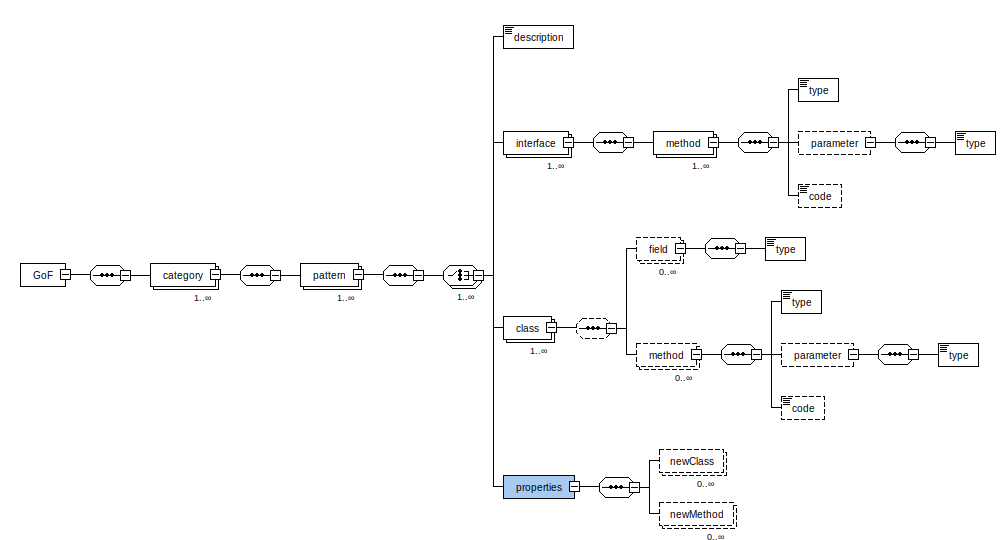
\includegraphics[width=1.0\textwidth]{Figures/xsd_diagram.png}
    \caption{Σχήμα αρχείου xml.}
    \label{fig:xsd}
\end{figure}
\newpage
\begin{lstlisting}[label=code:xml, caption=Περιγραφή μοτίβου Singleton.]
<pattern id="Singleton">
    <description>
        Ensure a class only has one instance, 
        and provide a global point of access to it.
    </description>
    <class id="Singleton" annotation="Singleton">
        <field id="instance" isStatic="true">
            <type>Singleton</type>
        </field>
        <method id="Singleton" visibility="private">
            <type></type>
        </method>
        <method id="getInstance" isStatic="true">
            <type>Object</type>
            <code>
                if (instance == null) {
                    instance = new Singleton();
                }
                return instance;
            </code>
        </method>
    </class>
</pattern>
\end{lstlisting}
\section{Αρχιτεκτονική}
\label{sec:packages}
\begin{figure}[H]
    \centering
    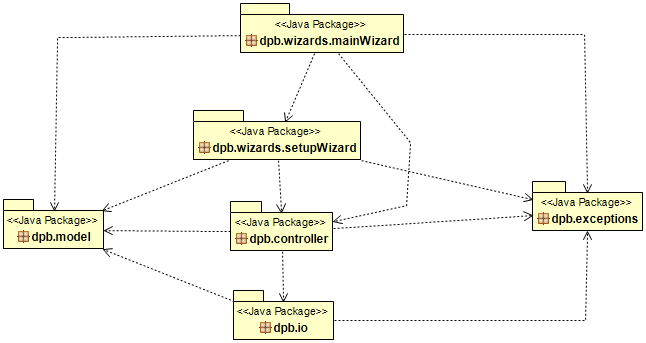
\includegraphics[width=1.0\textwidth]{Figures/packages.png}
    \caption{Διάγραμμα UML Πακέτων συστήματος.}
    \label{fig:packageUML}
\end{figure}
\begin{figure}[H]
    \centering
    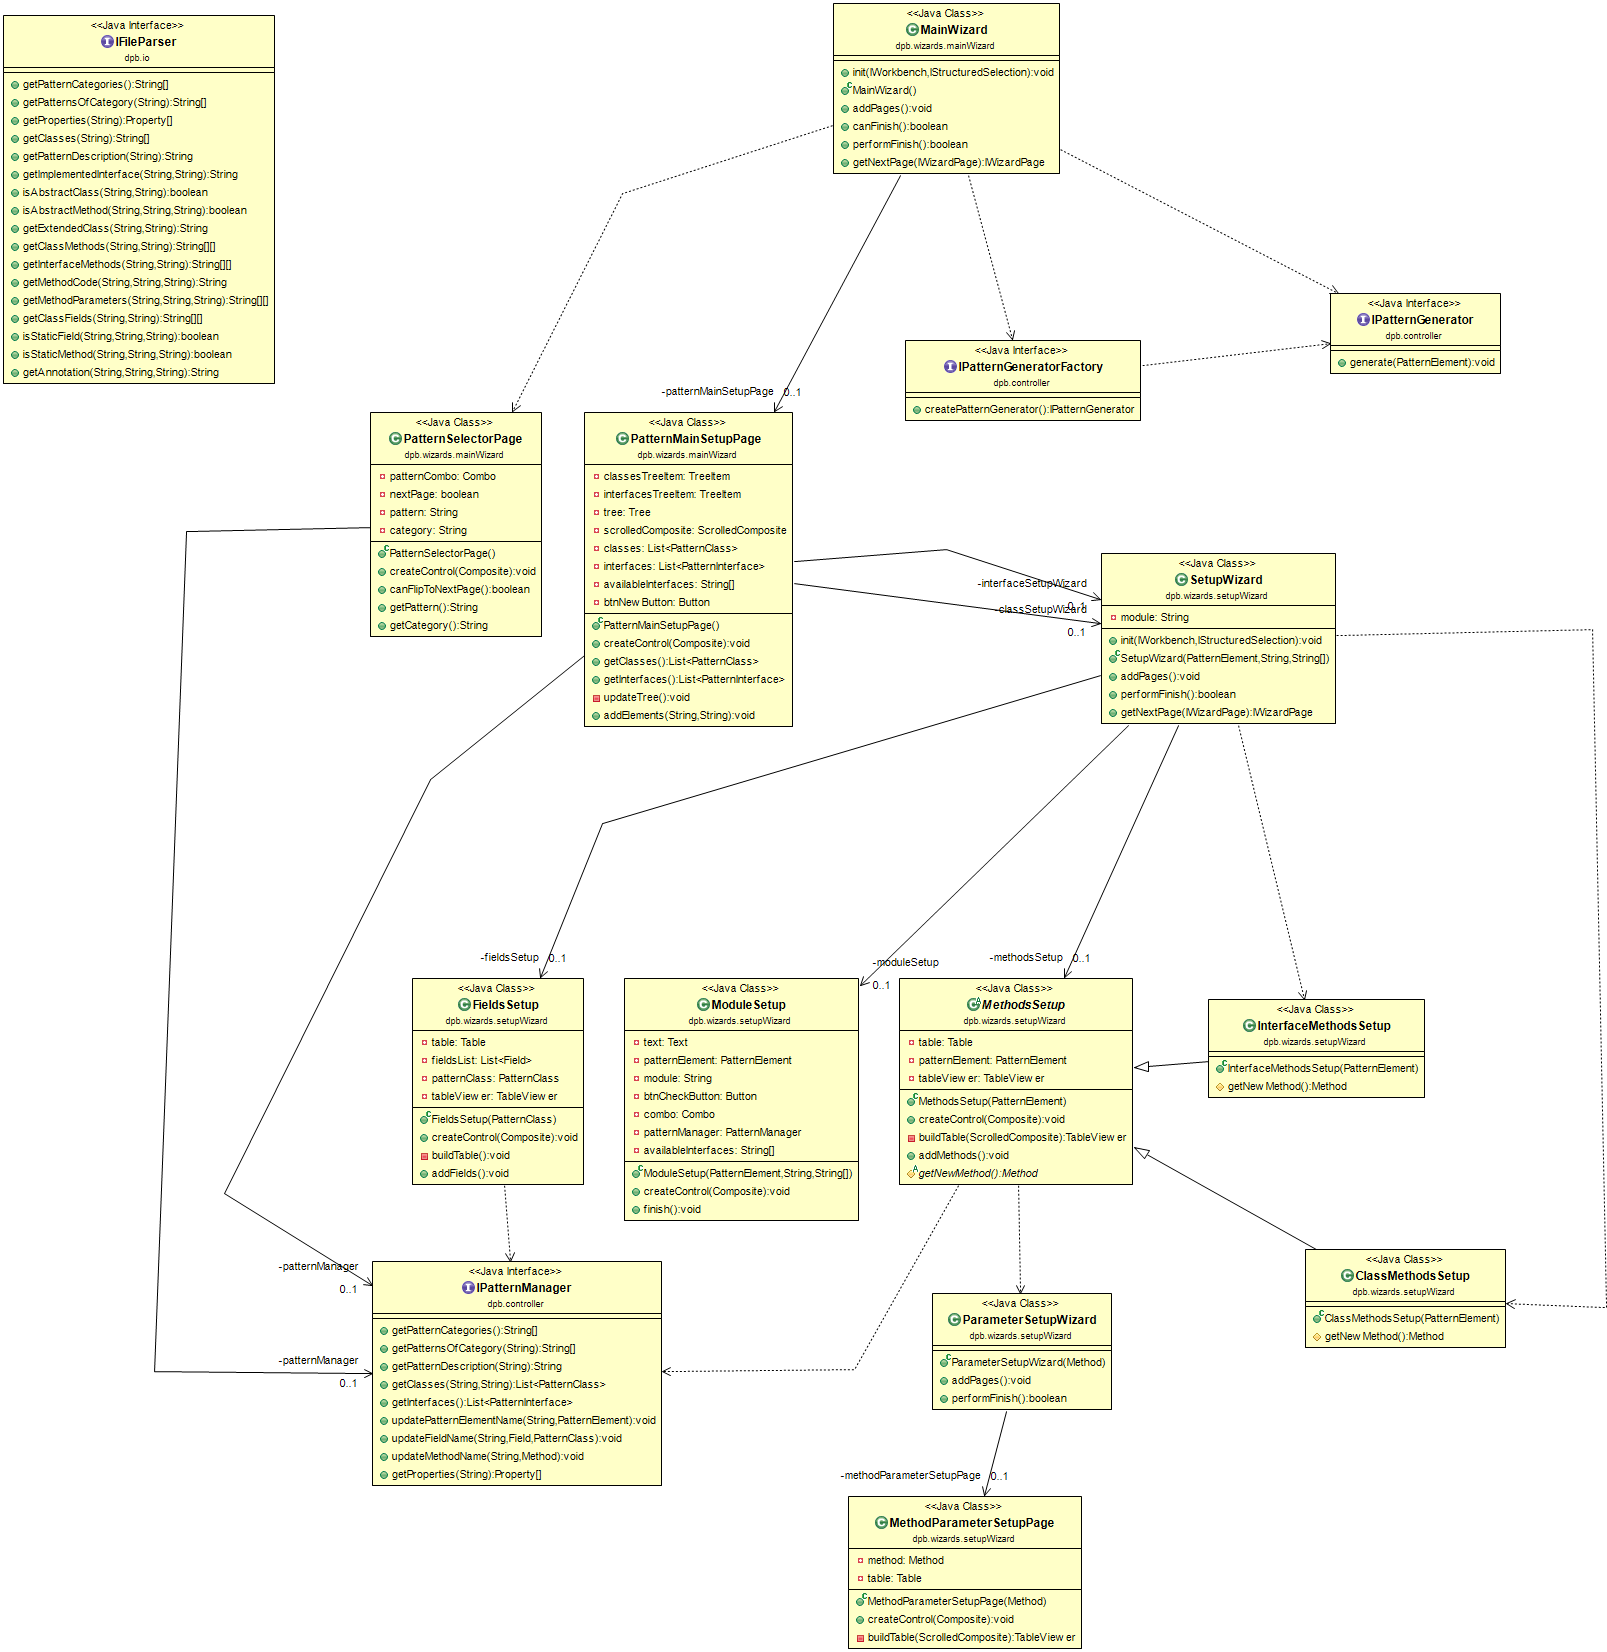
\includegraphics[width=1.0\textwidth]{Figures/system.png}
    \caption{Διάγραμμα UML κλάσεων \& διεπαφών συστήματος.}
    \label{fig:systemUML}
\end{figure}

Το λογισμικό αποτελείται από τα παρακάτω πακέτα,
\begin{itemize}
    \item dpb.wizards.mainWizard, σε αυτό το πακέτο, περιέχονται οι κλάσεις που αφορούν το γραφικό περιβάλλον του εργαλείου,
     πιο συγκεκριμένα, οι κλάσεις αυτού του πακέτου έχουν να κάνουν με την επιλογή του μοτίβου και την διαχείριση των κλάσεων και διεπαφών του 
     επιλεγμένου μοτίβου.
    \item dpb.wizards.setupWizards, σε αυτό το πακέτο, υπάρχουν οι κλάσεις που έχουν σχέση με την γραφική διεπαφή και την τροποποίηση των κλάσεων και διεπαφών, 
    όπως και των μεθόδων και πεδίων.
    \item dpb.controller, αποτελεί το πακέτο μέσω του οποίου η γραφική διεπαφή επικοινωνεί με το back-end. Χρησιμοποιεί τις λειτουργίες που παρέχει το back-end, 
    ώστε να  μετασχηματίζει τα ακατέργαστα δεδομένα των μοτίβων που παίρνει από το υποσύστημα io σε αντικείμενα κλάσεων που παρέχει το πακέτο model.
    \item dpb.io, αποτελεί το κομμάτι του συστήματος το οποίο χαρακτηρίζεται ως back-end.
     και είναι υπεύθυνο για το διάβασμα του αρχείου xml στο οποίο περιγράφονται τα μοτίβα. 
     Παρέχει λειτουργίες για την εισαγωγή των μοτίβων στο σύστημα.
    \item dpb.model, Το πακέτο αυτό, περιέχει τις κλάσεις οι οποίες αναπαριστούν τα αντικείμενα του πεδίου του προβλήματος.
    \item dpb.exceptions, Τέλος, στο πακέτο αυτό υπάρχουν κάποιες κλάσεις οι οποίες αναπαριστούν εξαιρέσεις 
        οι οποίες είναι κάποια γεγονότα που συμβαίνουν κατά την εκτέλεση του εργαλείου και διακόπτουν την κανονική ροή του προγράμματος.
\end{itemize}
% \newpage
% \section{Κλάσεις συστήματος}
% \label{sec:classes}
% \subsection{Ανάλυση κλάσεων}
% \label{subsec:classAnalysis}
% Παρακάτω, θα αναλύσουμε κάποιες βασικές κλάσεις του συστήματος,
% \begin{itemize}
%     \item PatternClass, η κλάση αυτή ανήκει στο πακέτο model και μοντελοποιεί μία κλάση του μοτίβου
%     \item PatternInterface, η κλάση αυτή ανήκει στο πακέτο model και μοντελοποιεί μία διεπαφή του μοτίβου
%     \item Method, η κλάση αυτή ανήκει στο πακέτο model και μοντελοποιεί μία μέθοδο που ανήκει σε κλάση ή διεπαφή του μοτίβου
%     \item Field, η κλάση αυτή ανήκει στο πακέτο model και μοντελοποιεί ένα πεδίο που ανήκει σε κλάση του μοτίβου
%     \item FileParser, είναι η βασική κλάση του υποσυστήματος io, είναι υπεύθυνη για το διάβασμα του αρχείου όπου περιγράφονται
%     τα μοτίβα και η βασική της δουλειά είναι να διαβάζει το αρχείο xml. Υποστηρίζει λειτουργίες όπως η ανάκτηση 
%     των κατηγοριών και των μοτίβων κάθε κατηγορίας, η ανάκτηση των κλάσεων και διεπαφών ενός μοτίβου, 
%     η ανάκτηση των annotations κάθε στοιχείου για κάποιο μοτίβο, όπως και οι ιδιότητες ενός μοτίβου 
%     οι οποίες είναι εάν επιτρέπεται η εισαγωγή νέας κλάσης, τέλος υποστηρίζει την ανάκτηση μεθόδων και πεδίων.
%     \item PatternManager, Μέσω της κλάσης αυτής παρέχεται η δυνατότητα στην γραφική διεπαφή του συστήματος 
%     να αντλεί οτιδήποτε χρειάζεται από το υποσύστημα io
%     \item PatternGenerator, Περιλαμβάνει την λειτουργία δημιουργίας των πηγαίων αρχείων στο πακέτο του έργου που έχει επιλέξει 
%     ο προγραμματιστής ή στο προεπιλεγμένο πακέτο, εάν δεν έχει επιλέξει κάποιο πακέτο, τα οποία περιέχουν 
%     τις κλάσεις του μοτίβου με τις μεθόδους και τα πεδία, όπως τα παραμετροποίησε ο προγραμματιστής, καθώς και τις διεπαφές. 
%     Επίσης προσθέτει στο classpath του έργου του προγραμματιστή το πακέτο που περιέχει τα annotations 
%     ώστε να είναι διαθέσιμα στον προγραμματιστή.
     
% \end{itemize}

\section{dpb.wizards.mainWizard}
\label{sec:dpb.wizards.mainWizard}
\begin{figure}[H]
    \centering
    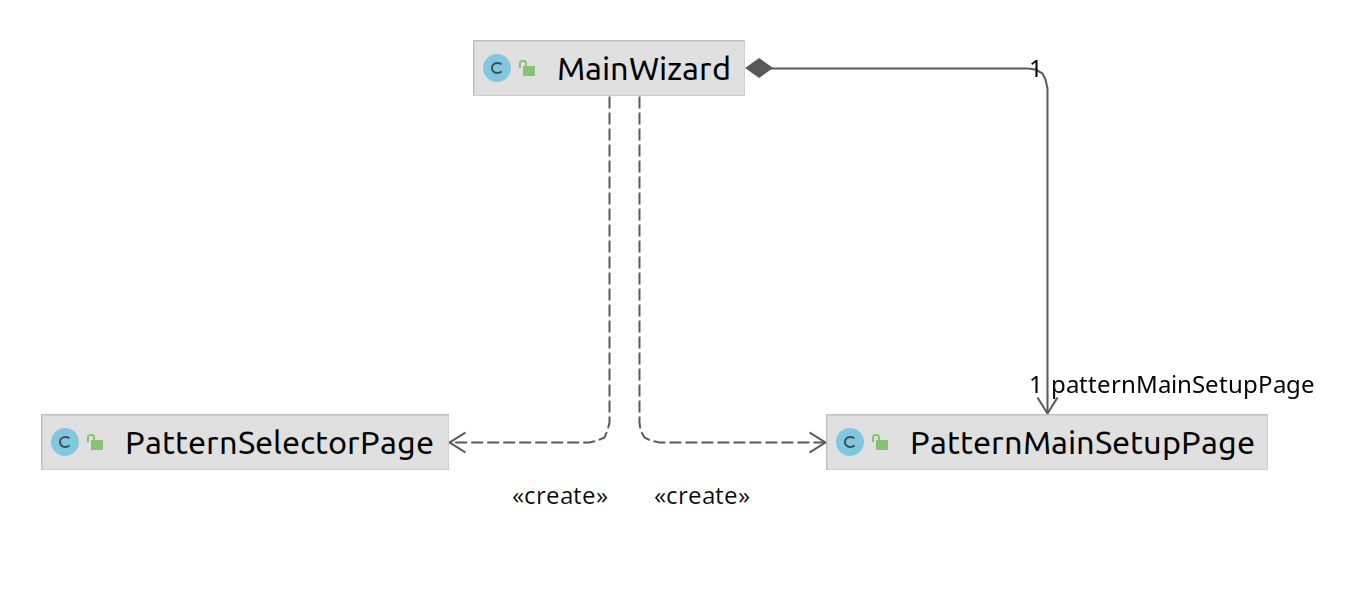
\includegraphics[width=1.0\textwidth]{Figures/mainWizard.png}
    \caption{Διάγραμμα UML Πακέτου mainWizard.}
    \label{fig:mainWizardUML}
\end{figure}
Το υποσύστημα αυτό, έχει να κάνει με τον κύριο οδηγό του εργαλείου, ο οποίος αποτελείται από δύο σελίδες. Η πρώτη σελίδα, 
δίνει στον προγραμματιστή την δυνατότητα να επιλέξει κατηγορία και μοτίβο. Στην δεύτερη σελίδα ο προγραμματιστής μπορεί να περιηγηθεί 
ανάμεσα στις διαθέσιμες κλάσεις και διεπαφές, καθώς και να προσθέσει κάποια καινούργια κλάση, 
εάν αυτό είναι δυνατό από τους περιορισμούς που ορίζονται στην περιγραφή των μοτίβων, 
όπως και να επεξεργαστεί τις κλάσεις και τις διεπαφές. η κλάση που υλοποιεί τον οδηγό, είναι η κλάση MainWizard, επεκτείνει την κλάση Wizard που παρέχει 
το Eclipse και υλοποιεί την διεπαφή INewWizard, η αρμοδιότητα της είναι να προσθέτει τις σελίδες του οδηγού αυτού, και να χειρίζεται 
το γεγονός κατά το οποίο προγραμματιστής έχει τελειώσει με την ρύθμιση του μοτίβου και κάνει κλικ στο κουμπί Τέλος, τότε καλείται η μέθοδος generate της κλάσης PatternGenerator,
για κάθε κλάση και διεπαφή του μοτίβου, η οποία θα αναλυθεί στην ενότητα \ref{sec:dpb.controller} και είναι υπεύθυνη για την παραγωγή των πηγαίων αρχείων.
Η κλάση PatternSelectonPage η οποία επεκτείνει την κλάση WizardPage και υλοποιεί την διεπαφή IWizardPage, 
είναι η πρώτη σελίδα του κύριου μας οδηγού, αυτό που κάνει είναι να χρησιμοποιεί την κλάση PatternManager, η οποία 
θα αναλυθεί στην ενότητα \ref{sec:dpb.controller}, ώστε να αντλήσει τις κατηγορίες των μοτίβων και να τις εμφανίσει σε μία λίστα, 
όταν επιλεχθεί μία κατηγορία από τον προγραμματιστή τότε ενεργοποιεί μία δεύτερη λίστα στην οποία προσθέτει 
τα μοτίβα αυτής της κατηγορίας. Τέλος η τελευταία κλάση του πακέτου αυτού είναι η κλάση PatternMainSetupPage 
η οποία και αυτή υλοποιεί και επεκτείνει αντίστοιχα τα IWizardPage και WizardPage, κύρια της δουλειά είναι η εμφάνιση των κλάσεων και διεπαφών 
του επιλεγμένου μοτίβου τα οποία αντλεί και αυτή με την χρήση του υποσυστήματος controller, και παρέχει κουμπιά για την προσθήκη νέας κλάσης, καθώς και 
την επεξεργασία των κλάσεων και διεπαφών, όταν ο χρήστης κάνει κλικ σε κάποιο κουμπί επεξεργασίας, τότε δημιουργείται 
ο δεύτερος οδηγός της γραφικής διεπαφής ο οποίος θα αναλυθεί στην ενότητα \ref{sec:dpb.wizards.setupWizards}.\newpage
\section{dpb.wizards.setupWizards}
\label{sec:dpb.wizards.setupWizards}
\begin{figure}[H]
    \centering
    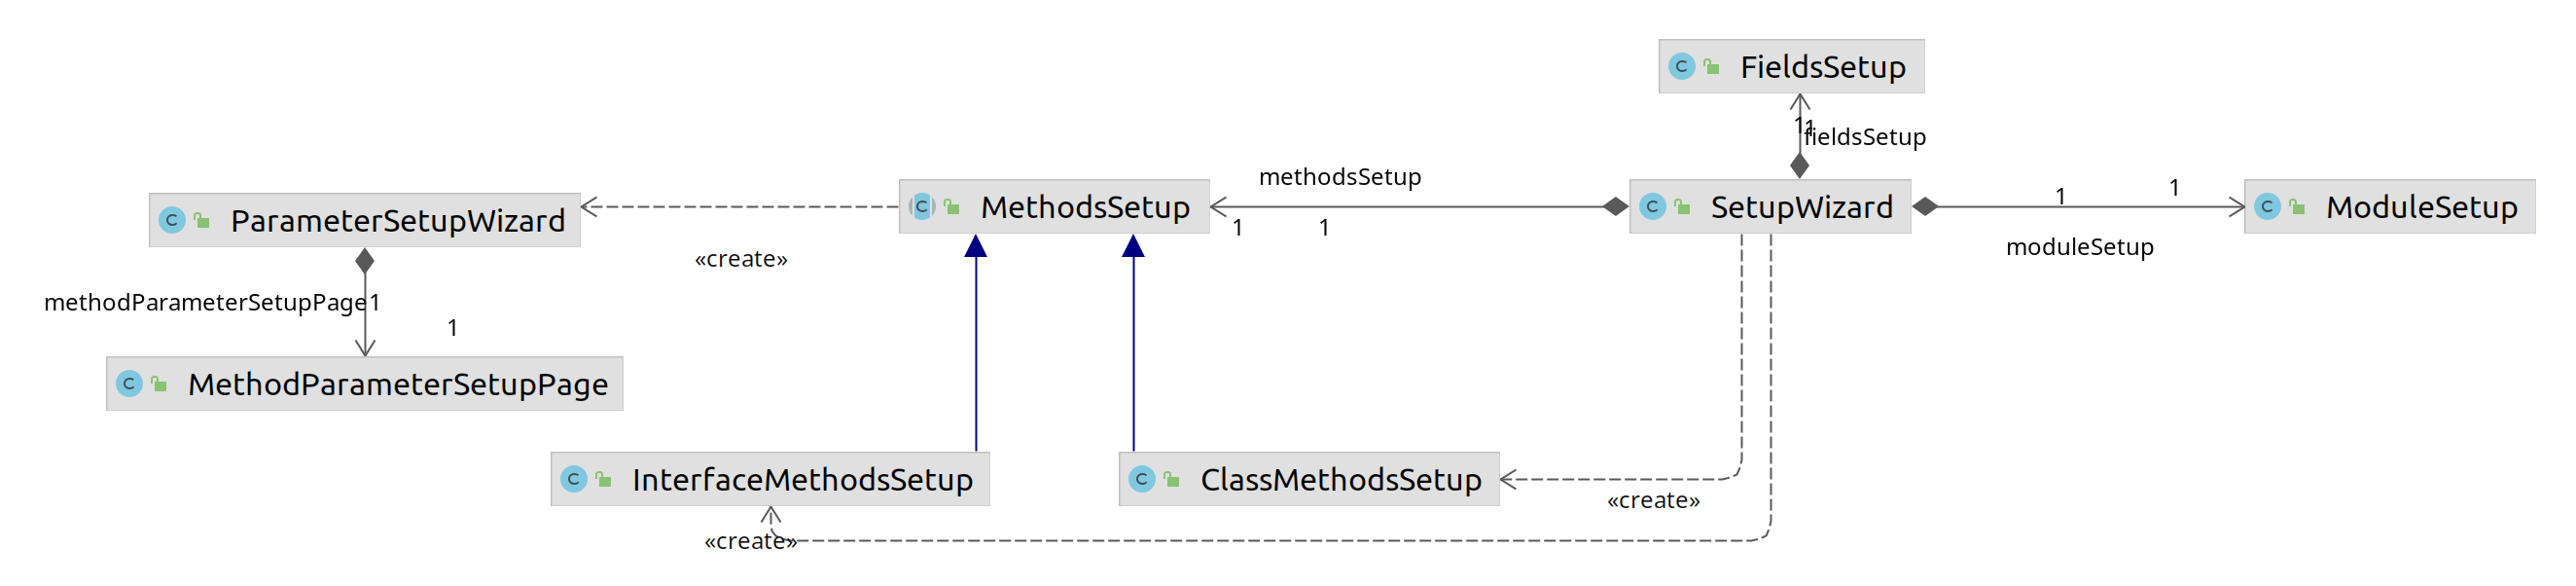
\includegraphics[width=1.0\textwidth]{Figures/setupWizard.png}
    \caption{Διάγραμμα UML Πακέτου setupWizards.}
    \label{fig:setupWizardUML}
\end{figure}
Το υποσύστημα αυτό, αποτελείται από δύο οδηγούς, ο πρώτος οδηγός είναι υπεύθυνος για την ρύθμιση των ονομάτων κλάσεων και διεπαφών, 
για την επιλογή κάποιας διεπαφής που θα υλοποιεί μία νέα κλάση, καθώς και για την ρύθμιση των πεδίων και μεθόδων. 
Η κλάση που υλοποιεί τον οδηγό αυτόν, είναι η κλάση SetupWizard, προσθέτει τις κατάλληλες σελίδες στον οδηγό, δηλαδή εάν ο προγραμματιστής 
θέλει να επεξεργαστεί μία κλάση τότε θα προσθέσει τρεις σελίδες, αλλιώς εάν επεξεργάζεται διεπαφή δύο σελίδες. 
Η τελευταία σελίδα είναι παρόμοια και για τις δύο περιπτώσεις, αφορά την επεξεργασία μεθόδων και υλοποιείται από την κλάση MethodsSetup,
Εμφανίζει στον προγραμματιστή όλες τις μεθόδους που ανήκουν στην κλάση ή διεπαφή που επεξεργάζεται αυτήν την στιγμή, 
ο προγραμματιστής έχει την δυνατότητα να αλλάξει το όνομα, την ορατότητα, καθώς και τον επιστρεφόμενο τύπο κάθε μεθόδου, 
επίσης έχει την δυνατότητα να προσθέσει ή διαγράψει κάποια μέθοδο, ακόμα μπορεί να επεξεργαστεί τις παραμέτρους κάποιας μεθόδου, 
για την λειτουργία αυτή, αναπτύχθηκε ακόμα ένας οδηγός ο οποίος υλοποιείται από την κλάση ParameterSetupWizard, 
έχει μία σελίδα, την MethodParameterSetup, η οποία εμφανίζει μία λίστα με τις παραμέτρους της επιλεγμένης μεθόδου και ο προγραμματιστής, 
έχει την δυνατότητα να αλλάξει το όνομα και τύπο κάθε παραμέτρου, καθώς και να προσθέσει ή διαγράψει κάποια παράμετρο. 
Μόλις ο χρήστης αλλάξει κάποια παράμετρο αυτομάτως ενημερώνεται και το αντικείμενο τύπου Parameter. 
Αντίστοιχα μόλις ο προγραμματιστής παραμετροποιεί κάποια μέθοδο τότε αυτομάτως ενημερώνεται και η δομή Method που αντιπροσωπεύει την μέθοδο αυτήν.
Ακόμα, και η πρώτη σελίδα είναι κοινή, υλοποιείται από την κλάση ModuleSetup, αλλά εάν πρόκειται για κλάση τότε περιέχει 
ένα κουμπί που ελέγχει εάν η κλάση θα είναι αφηρημένη και μία λίστα με τις διαθέσιμες διεπαφές που μπορεί να υλοποιήσει και οι δύο δυνατότητες 
είναι διαθέσιμες μόνο εάν πρόκειται για νέα κλάση. 
Η κλάση αυτή είναι υπεύθυνη και για τον χειρισμό του τερματισμού του οδηγού από το κουμπί Τέλος ή την μετάβαση σε επόμενη σελίδα, 
μόλις ο χρήστης πατήσει Τέλος ή επόμενο,  αντλούνται τα απαραίτητα δεδομένα από τα γραφικά στοιχεία εισόδου, 
που υπάρχουν στην σελίδα αυτή, όπως το όνομα, εάν είναι αφηρημένη κλάση, καθώς και το όνομα της διεπαφής που υλοποιεί, 
εάν πρόκειται για κλάση, και ενημερώνονται οι κατάλληλες δομές (PatternClass ή PatternInterface), τέλος, αναθέτουμε και το κατάλληλο annotation. 
Τέλος, έμεινε να αναλύσουμε την δεύτερη σελίδα της περίπτωσης όπου ο προγραμματιστής επεξεργάζεται κάποια κλάση, 
η σελίδα αυτή αφορά την επεξεργασία των πεδίων, υλοποιείται από την κλάση FieldsSetup, και είναι όμοια της σελίδας με τις μεθόδους, 
δηλαδή, εμφανίζονται σε μία λίστα όλα τα πεδία και ο χρήστης μπορεί να προσθέσει/διαγράψει κάποιο πεδίο, όπως και να αλλάξει την ορατότητα,
το όνομα και τον τύπο του πεδίου. Η ενημέρωση της σωστής δομής γίνεται και εδώ αμέσως μετά την επεξεργασία του πεδίου. 
Η διαφοροποιημένη συμπεριφορά στην επεξεργασία των μεθόδων για τις κλάσεις και τις διεπαφές, είναι στην λειτουργία προσθήκης νέας μεθόδου, 
και αναλυτικότερα στην δομή Method, η οποία δομή θα αναλυθεί στην ενότητα \ref{sec:dpb.model}, πιο συγκεκριμένα, 
αφορά  την παράμετρο του constructor της δομής αυτής, η οποία ορίζει εάν αυτή η μέθοδος ανήκει σε διεπαφή ή κλάση, 
οι μέθοδοι των διεπαφών έχουν το annotation της java, το @Override, όταν υλοποιούνται από κάποια κλάση 
και έτσι όταν ο χρήστης επεξεργάζεται κάποια διεπαφή, για να μην έχουμε διαφορετική κλάση που αναπαριστά σελίδα για την επεξεργασία μεθόδων διεπαφής, 
καθώς η υπόλοιπη λογική είναι ακριβώς ίδια, δημιουργήσαμε μία ιεραρχία κλάσεων, όπου η κλάση \mbox{ModuleSetup} είναι μία αφηρημένη κλάση, 
η οποία περιέχει την αφηρημένη μέθοδο για την προσθήκη νέας μεθόδου στην κλάση ή διεπαφή που μεταβάλει αυτήν την στιγμή ο προγραμματιστής, 
την κλάση αυτήν την επεκτείνουν, οι κλάσεις InterfaceMethodsSetup και ClassMethodsSetup, 
οι οποίες απλώς υλοποιούν την αφηρημένη μέθοδο με κατάλληλο τρόπο.
\section{dpb.controller}
\label{sec:dpb.controller}
\begin{figure}[H]
    \centering
    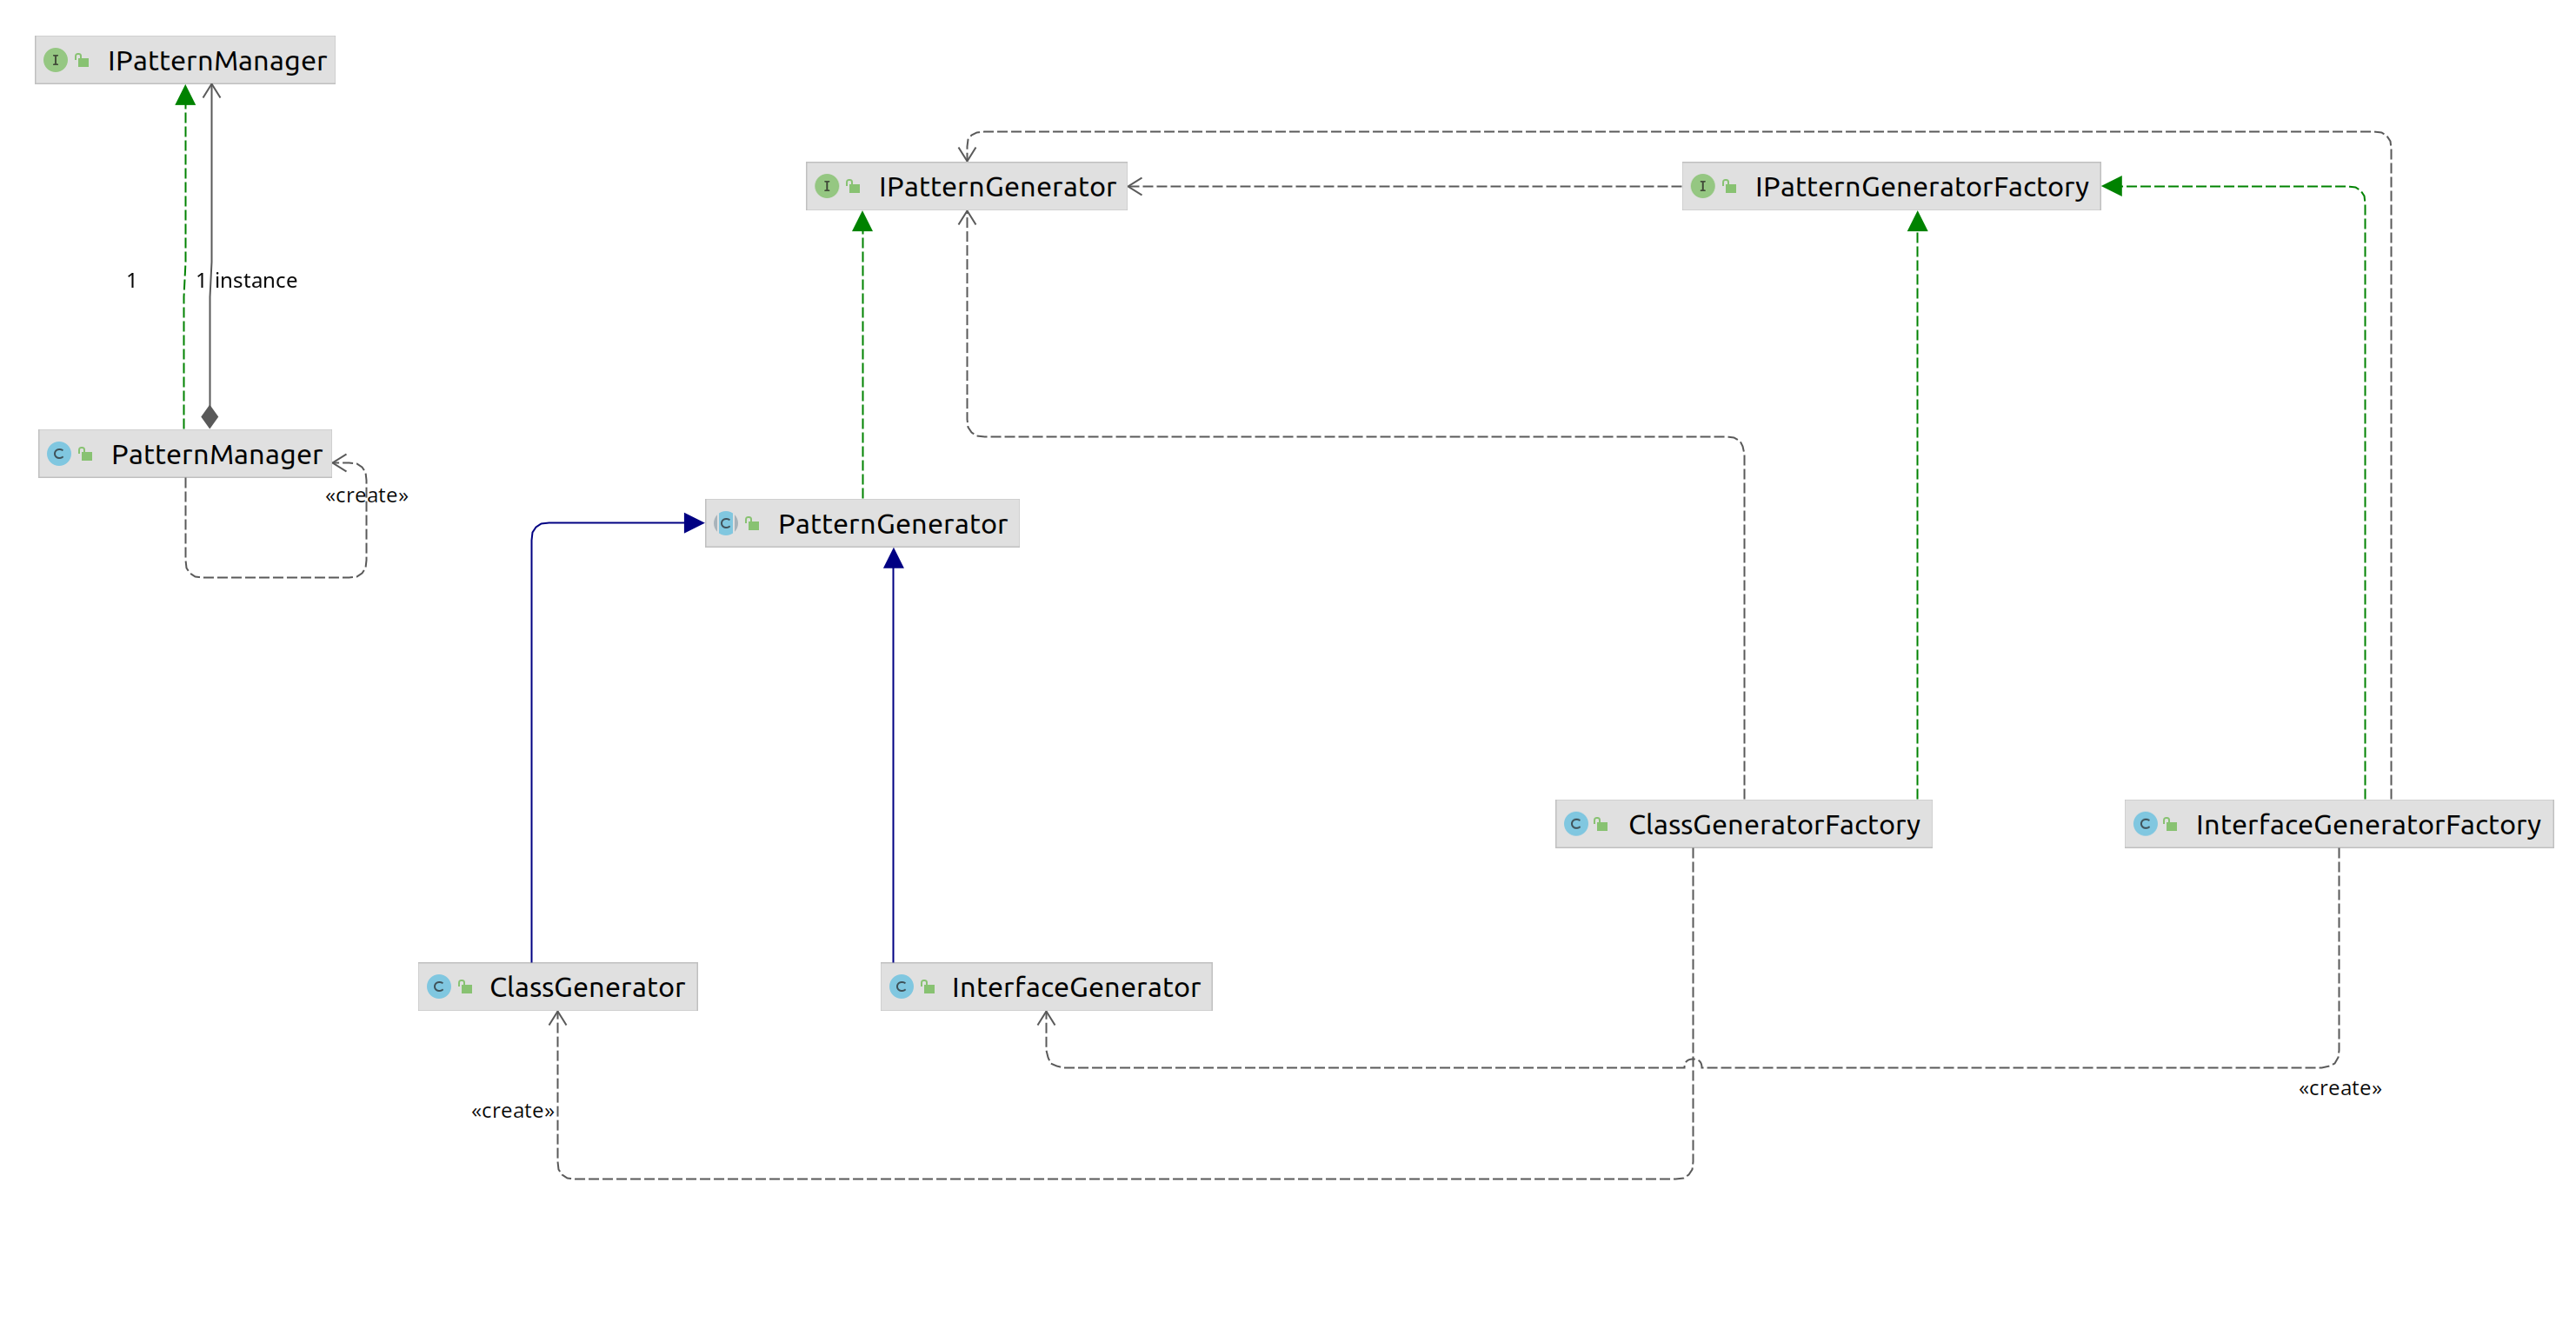
\includegraphics[width=1.0\textwidth]{Figures/controller.png}
    \caption{Διάγραμμα UML Πακέτου controller.}
    \label{fig:controllerUML}
\end{figure}
Το υποσύστημα του controller, είναι αρμόδιο για τις βασικές λειτουργίες του εργαλείου. Περιέχει την κλάση PatternManager, 
η οποία έχει ως σκοπό την παροχή των απαραίτητων πληροφοριών για κάποιο μοτίβο, καθώς και τα διαθέσιμα μοτίβα και κατηγορίες. 
Πιο συγκεκριμένα, δια μέσου αυτής της κλάσης η γραφική διεπαφή έχει διαθέσιμες τις δομές του πακέτου model, που 
περιγράφεται στην ενότητα \ref{sec:dpb.model}, δηλαδή, παρέχει ως πίνακες από Strings τις κατηγορίες και τα μοτίβα, τα οποία παίρνει 
από το υποσύστημα io της ενότητας \ref{sec:dpb.io}, και δημιουργεί αντικείμενα τύπου PatternClass αντλώντας το όνομα της κλάσης, 
την διεπαφή που υλοποιεί, τις μεθόδους και πεδία, καθώς και το εάν είναι αφηρημένη. Επίσης δημιουργεί αντικείμενα τύπου Method και Field, 
αντλώντας τις πληροφορίες από τον FileParser. Ακόμα, δημιουργεί και αντικείμενα τύπου PatternInterface, με όμοιο τρόπο, 
δηλαδή ανακτώντας το όνομα και τις μεθόδους από τον FileParser. Τέλος προσφέρει στο γραφικό περιβάλλον, μεθόδους για την σωστή ενημέρωση των ονομάτων.
\newline \newline
Στο υποσύστημα αυτό ανήκει και ιεραρχία κλάσεων για την δημιουργία των πηγαίων αρχείων java. δημιουργήσαμε αυτήν την ιεραρχία, καθώς,
ήταν απαραίτητο να εφαρμοστεί το μοτίβο Template Method \cite{GoF}, διότι η λειτουργία εξαγωγής των πηγαίων αρχείων χωρίστηκε σε κάποια βήματα, τα οποία είναι,
\begin{enumerate}
    \item Η προσθήκη του πακέτου που βρίσκεται η συγκεκριμένη κλάση ή διεπαφή του μοτίβου.
    \item Η προσθήκη των πεδίων μόνο στις κλάσεις. \label{enum:fields}
    \item Η προσθήκη των μεθόδων. \label{enum:methods}
    \item Η εξαγωγή του πηγαίου αρχείου που αφορά συγκεκριμένη κλάση ή διεπαφή του μοτίβου, με την χρήση του Eclipse API.
\end{enumerate}
Τα βήματα \ref{enum:fields} \& \ref{enum:methods}, είναι διαφορετικά για την περίπτωση που δημιουργούμε πηγαίο αρχείο κλάσης 
και διαφορετικό για την περίπτωση που δημιουργούμε πηγαίο αρχείο διεπαφής, καθώς οι διεπαφές δεν έχουν πεδία 
και οι μέθοδοι των διεπαφών δεν έχουν σώμα, Ακόμα διαφορά παρουσιάζει και ο ορισμός της διεπαφής και της κλάσης. 
Άρα κρίνεται απαραίτητη η χρήση του μοτίβου Template Method \cite{GoF}. Τέλος, η κλάση PatternGenerator, 
είναι υπεύθυνη και για την προσθήκη του πακέτου με τα annotations στο classpath του έργου του προγραμματιστή.
\newline \newline
Τέλος, για την μείωση της σύζευξης της ιεραρχίας IPatternGenerator με τα υπόλοιπα υποσυστήματα, 
χρησιμοποιήσαμε το μοτίβο Abstract Factory \cite{GoF}. Έτσι με αυτόν τον τρόπο τα υπόλοιπα υποσυστήματα, 
απλώς δημιουργούνε ένα \mbox{ClassGeneratorFactory} ή ένα \mbox{InterfaceGeneratorFactory}, 
και έτσι δημιουργούν έναν PatternGenerator ανάλογα την περίπτωση.
\section{dpb.io}
\label{sec:dpb.io}
\begin{figure}[H]
    \centering
    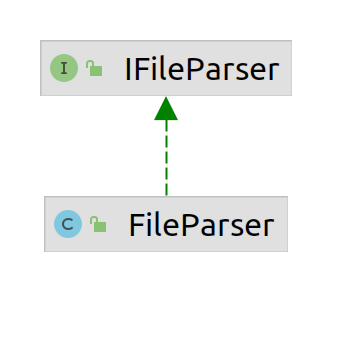
\includegraphics[width=1.0\textwidth]{Figures/io.png}
    \caption{Διάγραμμα UML Πακέτου io.}
    \label{fig:ioUML}
\end{figure}
Το υποσυστήματα αυτό, είναι το υποσύστημα που συνδέει το υπόλοιπο σύστημα με το αρχείο που περιγράφονται τα διάφορα μοτίβα. 
Η αρμοδιότητα του είναι αυτή ακριβώς, δηλαδή,  να διαβάζει το αρχείο xml και να μεταφέρει τις απαιτούμενες πληροφορίες στον controller. 
Αυτό που κάνει είναι να ανοίγει το αρχείο όπου περιγράφονται τα μοτίβα και να το διαβάζει. 
Είναι υπεύθυνο για την ανάκτηση των κατηγοριών και των μοτίβων, καθώς και την περιγραφή κάθε μοτίβου, 
επίσης διαβάζει και μεταβιβάζει με την μορφή συμβολοσειρών τα ονόματα των κλάσεων και διεπαφών, καθώς και τις ιδιότητες αυτών. Ακόμα, 
επιστρέφει το όνομα της διεπαφής που μπορεί να υλοποιεί μία κλάση, όπως, και το όνομα κάποιας κλάσης που μπορεί να επεκτείνει, 
και το αν μία κλάση είναι αφηρημένη. Επιστρέφει, το όνομα, την ορατότητα και τον επιστρεφόμενο τύπο, εάν είναι στατική η μέθοδος, 
όπως και τις παραμέτρους κάθε μεθόδου μίας διεπαφής ή κλάσης, επιπροσθέτως, εάν πρόκειται για κλάση επιστρέφει 
εάν η μέθοδος είναι αφηρημένη, καθώς και τον κώδικα που μπορεί να ορίζει κάποιο μοτίβο. Επιπλέον, 
διαβάζει το όνομα και τον τύπο κάθε πεδίου μίας κλάσης καθώς και εάν κάποιο πεδίο είναι στατικό.
Συμπληρωματικά, είναι υπεύθυνο, για την διαβίβαση κάποιων ιδιοτήτων των μοτίβων, όπως ποιες διεπαφές μπορεί 
να υλοποιεί κάποια νέα κλάση, καθώς και το εάν επιτρέπεται η προσθήκη νέας κλάσης και τέλος, τα annotations των νέων κλάσεων 
σύμφωνα με την διεπαφή που υλοποιούν. Τέλος, μεταβιβάζει στον controller και τα annotations που χαρακτηρίζουν μία κλάση ή διεπαφή του μοτίβου.
\section{dpb.model}
\label{sec:dpb.model}
\begin{figure}[H]
    \centering
    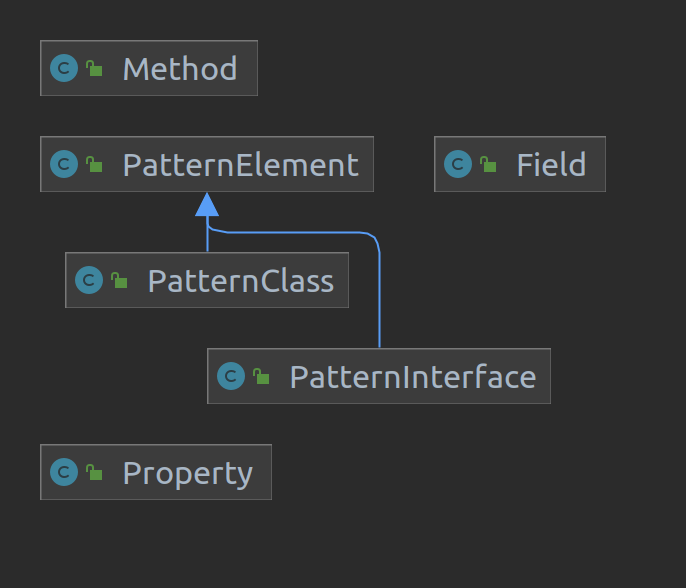
\includegraphics[width=1.0\textwidth]{Figures/model.png}
    \caption{Διάγραμμα UML Πακέτου model.}
    \label{fig:modelUML}
\end{figure}
Στο πακέτο αυτό, ορίζονται οι κλάσεις που αναπαριστούν τα αντικείμενα του πεδίου εφαρμογής.
\newline
Η κλάση Method αναπαριστά μία μέθοδο που ανήκει σε μία κλάση ή διεπαφή, έχει ως πεδία,
\begin{itemize}
    \item Το όνομα της μεθόδου.
    \item Τον επιστρεφόμενο τύπο της μεθόδου.
    \item Τον τροποποιητή της μεθόδου.
    \item Την λίστα των παραμέτρων της μεθόδου.
    \item Εάν είναι στατική μέθοδος.
    \item Εάν είναι αφηρημένη μέθοδος.
    \item Που ανήκει η μέθοδος.
    \item Τον κώδικα της μεθόδου.
    \item Εάν γίνεται Override η μέθοδος.
\end{itemize}
Ακόμα περιέχει getters \& setters και μία μέθοδο equal, για τον έλεγχο ισότητας με κάποιο άλλο αντικείμενο, 
καθώς χρειάζεται σε κάποιες περιπτώσεις.
\newline
Η κλάση Field αναπαριστά ένα πεδίο που ανήκει σε μία κλάση, έχει ως πεδία,
\begin{itemize}
    \item Το όνομα του πεδίου.
    \item Τον τύπο του πεδίου.
    \item Τον τροποποιητή του πεδίου.
    \item Εάν είναι στατικό πεδίο.
\end{itemize}
Αντίστοιχα και εδώ περιέχει getters \& setters και μία μέθοδο equal, για τον έλεγχο ισότητας με κάποιο άλλο αντικείμενο, 
καθώς χρειάζεται σε κάποιες περιπτώσεις.
\newline
Για την αναπαράσταση κλάσεων και διεπαφών, δημιουργήσαμε μία ιεραρχία, καθώς οι κλάσεις και οι διεπαφές 
έχουν πολλά κοινά χαρακτηριστικά, όπως, την κατηγορία μοτίβου και το μοτίβο που ανήκει μία κλάση/διεπαφή, το όνομα και την ορατότητα, 
καθώς και την λίστα με τις μεθόδους. Εκτός των κοινών χαρακτηριστικών έχουν και κάποιες διαφορές, για αυτόν τον λόγο προκύπτει η ανάγκη, 
να δημιουργήσουμε μία μαμά κλάση που θα έχει τα κοινά χαρακτηριστικά τους, και δύο κλάσεις που κληρονομούν την μαμά κλάση PatternElement, 
την κλάση PatternClass, η οποία αντιπροσωπεύει μία κλάση του μοτίβου και την PatternInterface που αντιπροσωπεύει μία διεπαφή του μοτίβου. 
Η κλάση PatternClass, περιέχει ως πεδία, την διεπαφή που υλοποιεί, την κλάση που επεκτείνει, εάν είναι αφηρημένη και 
μία λίστα με τα πεδία που έχει κάποια κλάση του μοτίβου. Ενώ η κλάση PatternInterface έχει ως μοναδικό 
πεδίο μία λίστα με τις κλάσεις που υλοποιούν την συγκεκριμένη διεπαφή, ώστε να μπορούμε να προσθέσουμε τις μεθόδους της 
διεπαφής στις κλάσεις που την υλοποιούν. Τέλοςμ εκτός από τις μεθόδους get \& set, έχουμε δημιουργήσει και μεθόδους 
οι οποίες προσθέτουν μία μέθοδο σε μία διεπαφή ή κλάση του μοτίβου, όπως και μεθόδους για την αφαίρεση κάποιας μεθόδου.
\newline
Τέλος, έμεινε η κλάση Property, η οποία απλώς αναπαριστά τις ιδιότητες κάθε μοτίβου που έχουμε παρουσιάσει παραπάνω. Η κλάση αυτή, 
έχει δύο πεδία, το ένα πεδίο αφορά το annotation που θα έχει κάποια καινούργια κλάση/διεπαφή που υλοποιεί/επεκτείνει, 
κάποια διεπαφή ή άλλη κλάση και το δεύτερο πεδίο αφορά την κλάση/διεπαφή που μπορεί να επεκτείνει/υλοποιεί η  νέα κλάση. Σαν μεθόδους έχει απλώς, 
getters \& setters.

\chapter{Έλεγχος}
\label{ch:testing}
Στο κεφάλαιο αυτό θα αναλυθούν οι έλεγχοι που υλοποιήθηκαν για τον κώδικα της εφαρμογής. 
Ο έλεγχος χωρίστηκε σε δύο επιμέρους κατηγορίες, στον έλεγχο του εργαλείου και στον έλεγχο των μοτίβων που υλοποιεί το εργαλείο.
Για την υλοποίησή τους χρησιμοποιήθηκε η βιβλιοθήκη Junit 4.
\section{Έλεγχος δομής σχεδιαστικών μοτίβων}
\label{sec:patternTesting}
\subsection{Έλεγχος μεθόδων φορτώματος μοτίβων}
\label{subsec:patternManagerTesting}
Σε αυτήν την ενότητα, θα παρουσιαστούν οι έλεγχοι για την δομή των μοτίβων τα οποία περιγράφονται σε ένα αρχείο xml.
Για να επιβεβαιώσουμε την σωστή δομή κάθε μοτίβου, το μόνο που χρειάζεται είναι να ελέγξουμε την κλάση η οποία δημιουργεί 
τα απαραίτητα αντικείμενα αντλώντας δεδομένα από το αρχείο περιγραφής των μοτίβων, κλάση αυτή είναι η PatternManager.
Έχουμε δημιουργήσει τεστ τα οποία ελέγχουν εάν οι κλάσεις κάθε μοτίβου, έχουν το σωστό όνομα, υλοποιούν ή επεκτείνουν την σωστή 
διεπαφή ή κλάση αντίστοιχα και περιέχουν τις σωστές μεθόδους και πεδία. Επίσης υπάρχουν τεστ τα οποία επιβεβαιώνουν την δομή των 
διεπαφών, ελέγχοντας το όνομα και τις μεθόδους κάθε διεπαφής. Οι περιπτώσεις ελέγχων χωρίστηκαν σε δύο πακέτα, 
στο ένα πακέτο υπάρχουν οι περιπτώσεις ελέγχου των κλάσεων κάθε μοτίβου, και στο άλλο πακέτο υπάρχουν οι περιπτώσεις ελέγχου 
των διεπαφών κάθε μοτίβου. Πιο συγκεκριμένα, οι περιπτώσεις ελέγχου κατηγοριοποιούνται σύμφωνα με την 
κατηγορία των μοτίβων που έχουν προτείνει οι GoF \cite{GoF}. Στο πακέτο dpb.patternManagerTests.getClassTests, υπάρχουν οι εξής περιπτώσεις ελέγχου:
\begin{itemize}
    \item TestGetClassCreational, Τα τεστ αυτής της κλάσης ελέγχουν όλα τα μοτίβα της κατηγορίας creational
    \item TestGetClassStructural, Τα τεστ αυτής της κλάσης ελέγχουν όλα τα μοτίβα της κατηγορίας structural
    \item TestGetClassBehavioral, Τα τεστ αυτής της κλάσης ελέγχουν όλα τα μοτίβα της κατηγορίας behavioral
\end{itemize}
Για να επιβεβαιώσουμε την δομή κάθε μοτίβου, καλούμε την μέθοδο getClass(String, String), η οποία μας επιστρέφει 
μία λίστα με τις κλάσεις του συγκεκριμένου μοτίβου, για κάθε κλάση ελέγχουμε το όνομα της και αν υλοποιεί κάποια διεπαφή, 
το όνομα της διεπαφής, αντίστοιχα εάν επεκτείνει κάποια άλλη κλάση. Στη συνέχεια ελέγχουμε για κάθε πεδίο το όνομα του και 
τον τύπο του. Τέλος για κάθε μέθοδο ελέγχουμε το όνομα της, τον επιστρεφόμενο τύπο, 
το όνομα και τον τύπο κάθε παραμέτρου και το σώμα της μεθόδου εάν υπάρχει.
\linebreak
Στο πακέτο dpb.patternManagerTests.getInterfaceTests, υπάρχουν οι εξής περιπτώσεις ελέγχου:
\begin{itemize}
    \item TestGetInterfaceCreational, Τα τεστ αυτής της κλάσης ελέγχουν όλα τα μοτίβα της κατηγορίας creational
    \item TestGetInterfaceStructural, Τα τεστ αυτής της κλάσης ελέγχουν όλα τα μοτίβα της κατηγορίας structural
    \item TestGetInterfaceBehavioral, Τα τεστ αυτής της κλάσης ελέγχουν όλα τα μοτίβα της κατηγορίας behavioral
\end{itemize}
Για να επιβεβαιώσουμε την δομή κάθε μοτίβου, καλούμε την μέθοδο getClass(String, String), η οποία μας επιστρέφει 
μία λίστα με τις κλάσεις του συγκεκριμένου μοτίβου και στην συνέχεια την μέθοδο getInterfaces(), για κάθε διεπαφή 
ελέγχουμε το όνομα της. Στη συνέχεια για κάθε μέθοδο ελέγχουμε το όνομα της, τον επιστρεφόμενο τύπο και
το όνομα και τον τύπο κάθε παραμέτρου.
\subsection{Έλεγχος μεθόδου ανάκτησης περιγραφής μοτίβου}
\label{subsec:getDescriptionTest}
Για τον έλεγχο της μεθόδου getPatternDescription(String) που ανήκει στην κλάση dpb.controller.PatternManager, υλοποιήσαμε την τεστ κλάση
TestGetDescription, η οποία έχει τρεις περιπτώσεις ελέγχου, μία για κάθε κατηγορία. Για κάθε μοτίβο κάθε κατηγορίας,
απλώς επιβεβαιώνουμε την περιγραφή του μοτίβου καλώντας την getPatternDescription και ελέγχοντας εάν είναι η αναμενόμενη περιγραφή.
\section{Έλεγχος μεθόδων δημιουργίας πηγαίου κώδικα java}
\label{sec:patternGeneratorTesting}
Η ενότητα αυτή, έχει σκοπό να παρουσιάσει τους ελέγχους της μεθόδου η οποία είναι υπεύθυνη 
για την δημιουργία των πηγαίων αρχείων java που περιέχουν τις κλάσεις και τις διεπαφές του μοτίβου μαζί με τις 
διάφορες παραμετροποιήσεις που μπορεί να έχει κάνει ο προγραμματιστής. Η μέθοδος η οποία είναι υπεύθυνη για την εξαγωγή 
του πηγαίου κώδικα είναι η μέθοδος generate(PatternElement) που ορίζεται στην διεπαφή dpb.controller.IPatternGenerator. 
Δεν χρειάζεται να ελέγξουμε την μέθοδο generate εξονυχιστικά για κάθε μοτίβο καθώς, γνωρίζουμε την ορθότητα των μοτίβων από τα τεστ που 
περιγράφηκαν στην προηγούμενη ενότητα \ref{subsec:patternManagerTesting}, παρά μόνο για ένα τυχαίο μοτίβο, 
διαλέξαμε το μοτίβο Singleton της κατηγορίας creational καθώς έχει απλή δομή. Για την υλοποίησή των ελέγχων χρειάστηκε να δημιουργήσουμε
μερικά mock αντικείμενα \cite{SWEBOK}, διότι η μέθοδος generate έχει πεδίο ένα αντικείμενο τύπου IPackageFragment, 
το οποίο κατά την φάση του ελέγχου έχει τιμή null, καθώς αυτό το αντικείμενο αναπαριστά το πακέτο που έχει επιλέξει ο προγραμματιστής 
για την εξαγωγή όλων των πηγαίων αρχείων. Επίσης είναι απαραίτητο να κάνουμε faking \cite{SWEBOK} και την κλάση που υλοποιεί
την διεπαφή IPatternGenerator, καθώς κατά την δημιουργία ενός αντικειμένου της κλάσης αυτής καλείται 
η μέθοδος addAnnotationsToClassPath() η οποία κατά τον έλεγχο δεν είναι απαραίτητη καθώς προσθέτει στο classpath του εκάστοτε έργου 
τα annotations. Για την κατασκευή των fake αντικειμένων \cite{SWEBOK}, απλώς κάναμε override τις απαραίτητες μεθόδους.
Δηλαδή, για την περίπτωση της ClassGenerator, υλοποιήσαμε μία νέα κλάση στο πακέτο που έχουμε τους ελέγχους, 
η οποία επεκτείνει την κλάση ClassGenerator, και απλώς υλοποιεί την μέθοδο addAnnotationsToClassPath(), όπως φαίνεται στο παράδειγμα 
\ref{code:ClassGenerator}. Για την κατασκευή του fake αντικειμένου \cite{SWEBOK} IPackageFragment, 
δημιουργήσαμε μία κλάση η οποία υλοποιεί την διεπαφή IPackageFragment, η κλάση αυτή έχει τρία πεδία τα οποία αναπαριστούν 
το όνομα του παραγόμενου πηγαίου αρχείου, τον κώδικα του αρχείου αυτού και το όνομα του πακέτου που θα εξαχθεί το πηγαίο αρχείο. 
Επίσης, τροποποιούμε την μέθοδο getElementName ώστε να επιστρέφει το πεδίο με το όνομα του πακέτου την createCompilationUnit, 
ώστε να θέτει το όνομα και τον κώδικα του πηγαίου αρχείου και τέλος, προσθέτουμε δύο getters για το όνομα και τον κώδικα, 
ώστε να μπορούμε να επαληθεύσουμε αργότερα την ορθή λειτουργία της παραγωγής κώδικα όπως φαίνεται στο παράδειγμα 
\ref{code:mockPackage}. Τέλος, η κλάση για τον έλεγχο είναι η dpb.patternGeneratorTests.GenerateTests. 
Αφού, έχουμε δημιουργήσει τα απαραίτητα mock αντικείμενα \cite{SWEBOK}, 
καλούμε την μέθοδο generate με παράμετρο την μοναδική κλάση του μοτίβου Singleton και επιβεβαιώνουμε 
την ορθή λειτουργία της μεθόδου generate ελέγχοντας τι επιστρέφουν οι getters.
\newpage
\begin{lstlisting}[label=code:ClassGenerator, caption=Mock κλάση για την κλάση ClassGenerator, language=java]
package dpb.patternGeneratorTests;

import java.io.IOException;
import java.net.URISyntaxException;

import org.eclipse.core.runtime.CoreException;
import org.eclipse.jdt.core.JavaModelException;

import dpb.controller.ClassGenerator;

public class MockClassGenerator extends ClassGenerator {

    public MockClassGenerator() throws CoreException, URISyntaxException, IOException {
        super();
        // TODO Auto-generated constructor stub
    }

    @Override
    protected void addAnnotationsToClassPath() throws JavaModelException, URISyntaxException, IOException {
        // TODO Auto-generated method stub
    }
}
\end{lstlisting}
\newpage
\begin{lstlisting}[label=code:mockPackage, caption=Mock κλάση για την κλάση PackageFragment, language=java]
public class MockPackageFragment implements IPackageFragment {
    private final String elementName;
    private String arg0;
    private String arg1;
            
    public MockPackageFragment(String elementName) {
        this.elementName = elementName;
    }

    @Override
    public String getElementName() {
        return elementName;
    }

    @Override
    public ICompilationUnit createCompilationUnit(String arg0, String arg1, boolean arg2, IProgressMonitor arg3)
            throws JavaModelException {
        this.arg0 = arg0;
        this.arg1 = arg1;
        return null;
    }


    public String getArg0() {
        return arg0;
    }

    public String getArg1() {
        return arg1;
}
\end{lstlisting}
    


\section{Λοιποί έλεγχοι}
\label{sec:moreTests}
Τέλος, δημιουργήθηκαν μερικά ακόμα τεστ, για την επαλήθευση κάποιων μεθόδων τα οποία τεστ περιγράφουμε παρακάτω,
\begin{itemize}
    \item testGetPatternCategories, το τεστ αυτό επαληθεύει τις διαθέσιμες κατηγορίες μοτίβων που εμφανίζονται στον χρήστη
    \item testGetPatternsOfCategory, το τεστ αυτό επαληθεύει τα μοτίβα κάποιας κατηγορίας που είναι διαθέσιμα στον προγραμματιστή
    \item testUpdatePatternElementName, το τεστ αυτό επαληθεύει την λειτουργία αλλαγής ονόματος μίας κλάσης ή διεπαφής
    \item testUpdateFieldName, το τεστ αυτό επαληθεύει την λειτουργία αλλαγής ονόματος ενός πεδίου
    \item testUpdateMethodName, το τεστ αυτό επαληθεύει την λειτουργία αλλαγής ονόματος κάποιας μεθόδου
    \item testGetProperties, το τεστ αυτό επαληθεύει τις ιδιότητες ενός μοτίβου, οι οποίες είναι, εάν το μοτίβο επιτρέπει την προσθήκη
    νέας κλάσης, ποίες διεπαφές μπορεί να υλοποιήσει μία νέα κλάση και τέλος το annotation κάθε κλάσης ή διεπαφής
\end{itemize}
\section{Αναφορά αποτελεσμάτων ελέγχων}
\label{sec:testReport}
\begin{figure}[H]
    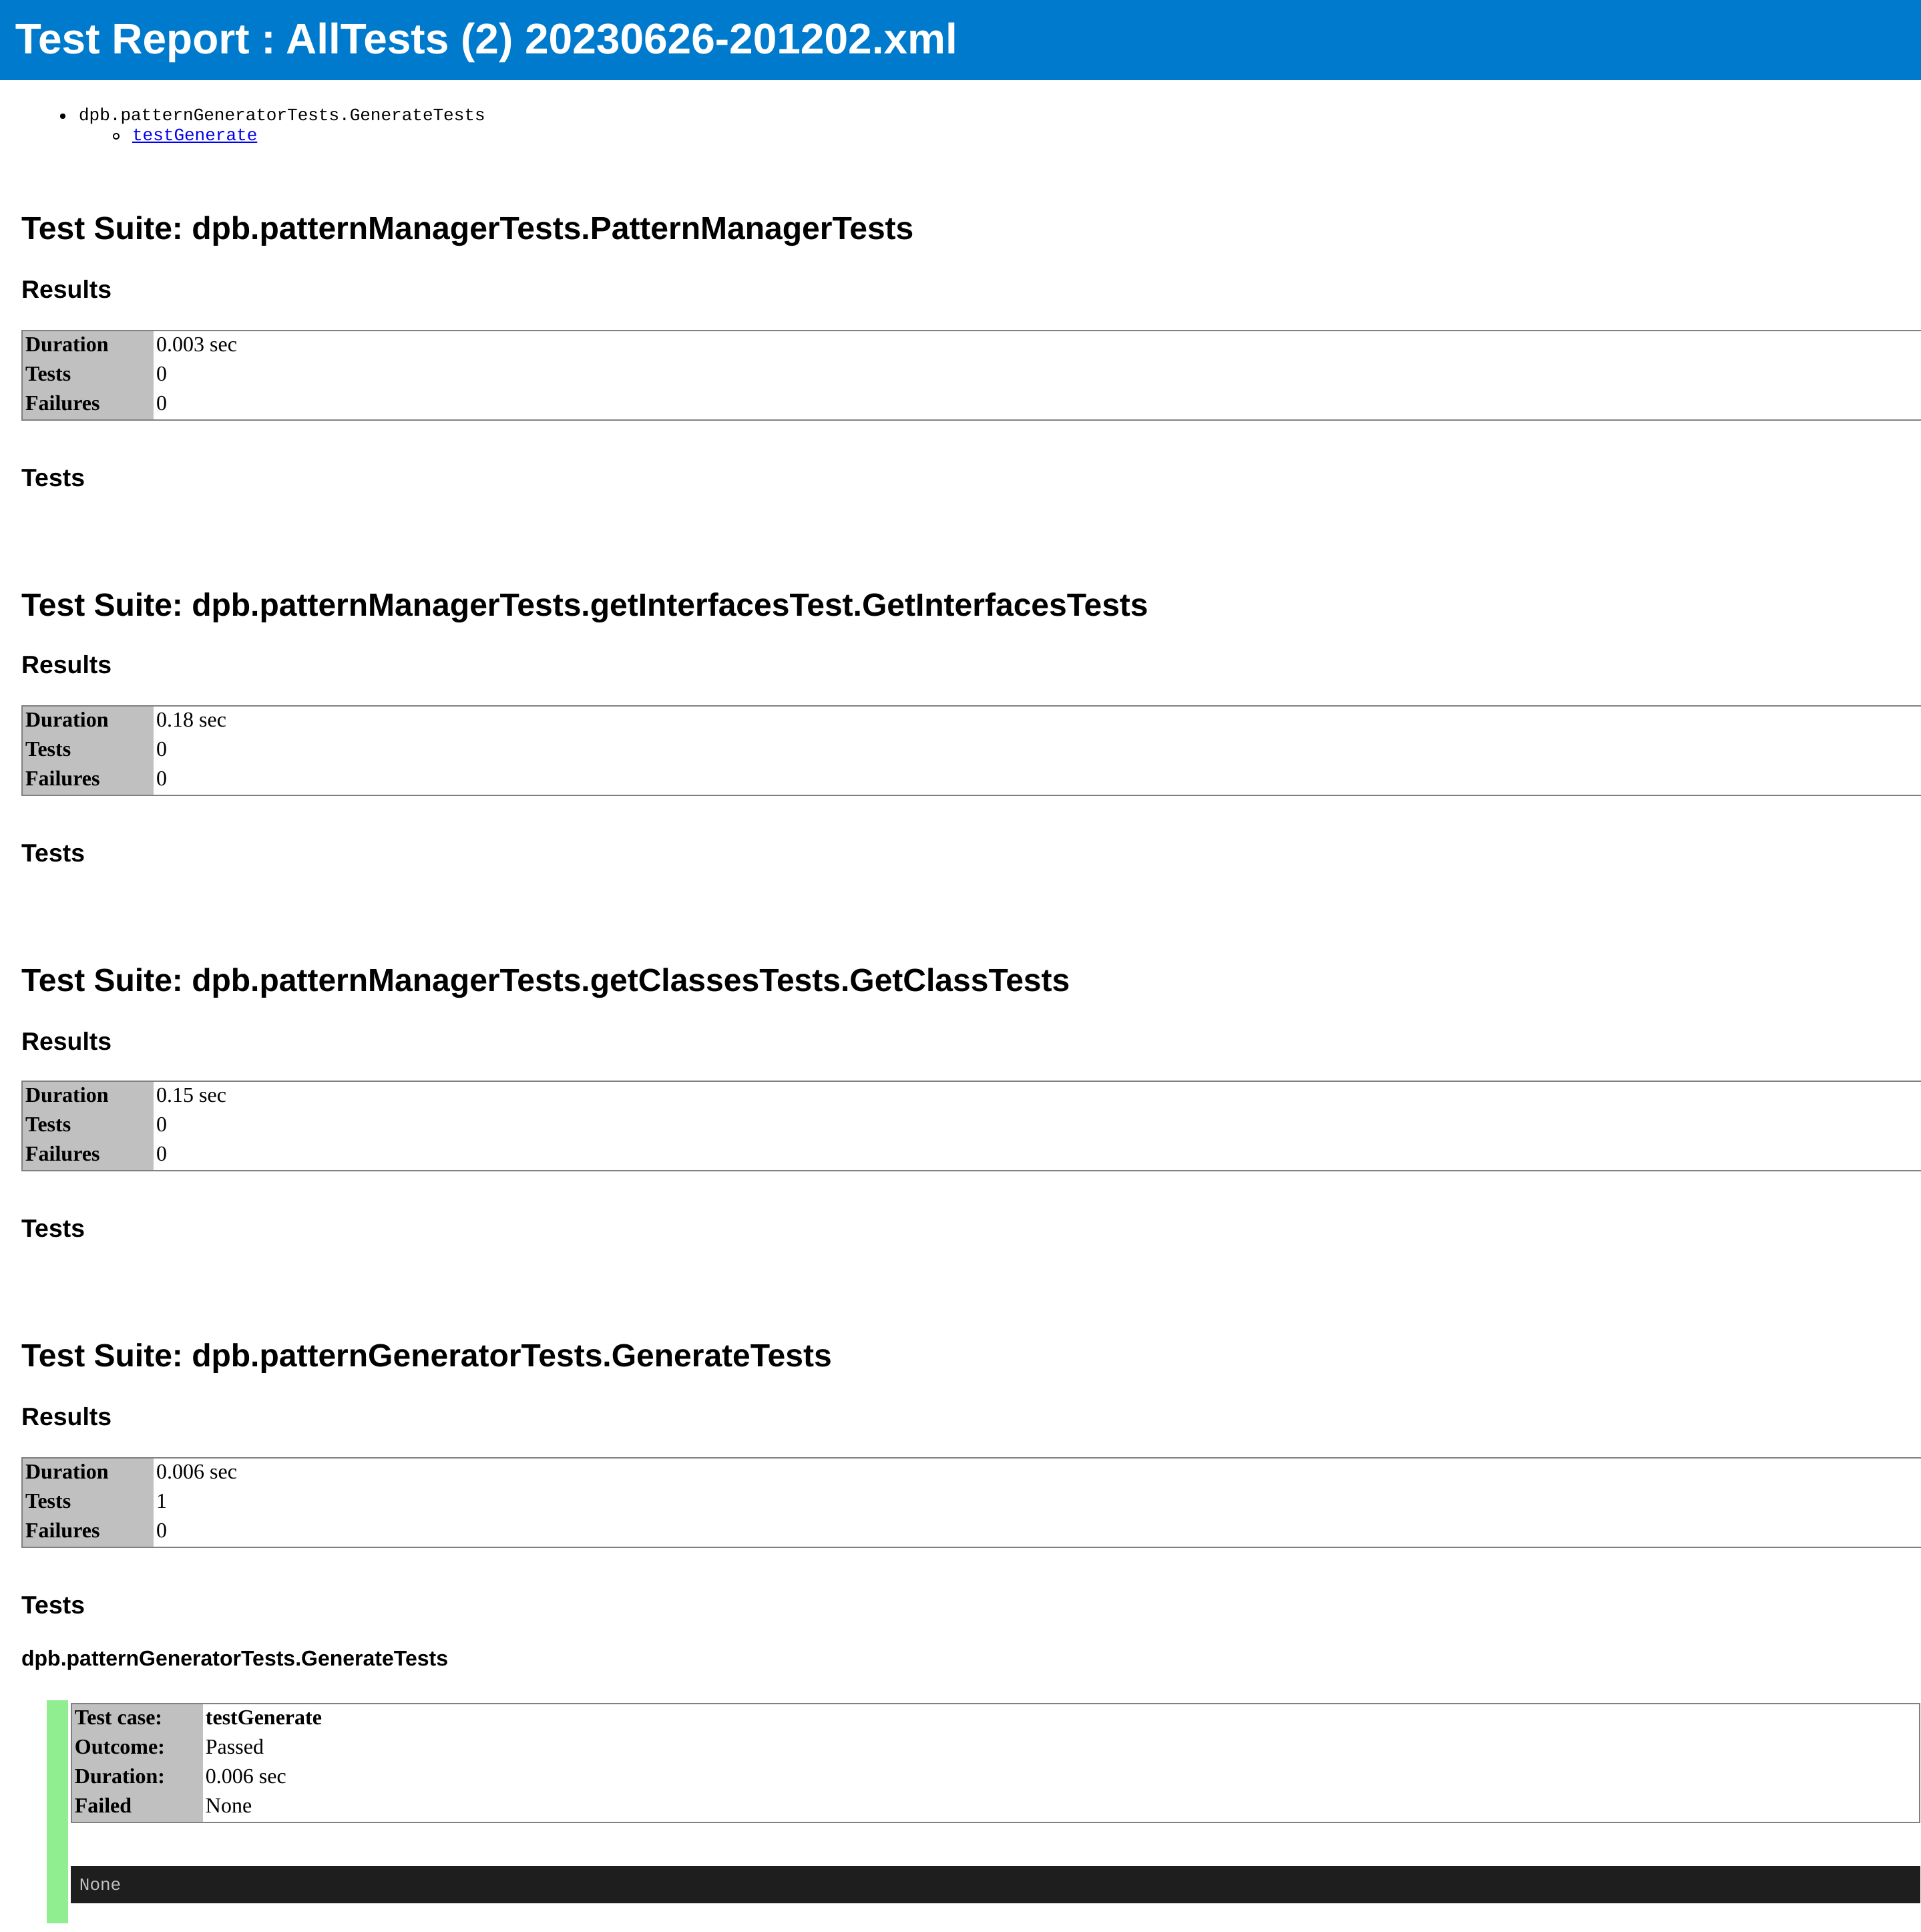
\includegraphics[width=1.0\textwidth]{Figures/test_report.png}
    \label{fig:testReport}
    \caption{Αναφορά αποτελεσμάτων ελέγχων}
\end{figure}
\chapter{Οδηγός Χρήσης Design Pattern Builder}
\label{ch:manual}


\section{Λειτουργίες χρήστη}
\label{sec:manual}
Για να μπορεί να χρησιμοποιήσει ένας προγραμματιστής το Design Pattern Builder, θα πρέπει να επιλέξει το πακέτο που επιθυμεί να εισάγει 
ένα μοτίβο ή το τρέχων έργο στο οποίο εργάζεται, να κάνει δεξί κλικ, να επιλέξει New και στην καρτέλα 
Other θα βρει την επιλογή Design Pattern Builder, όπως φαίνεται στην εικόνα \ref{fig:open_wizard}, 
αφού επιλέξει Import Pattern θα εμφανιστεί ο οδηγός της εικόνας \ref{fig:select_pattern}.
\begin{figure}[H]
    \centering
    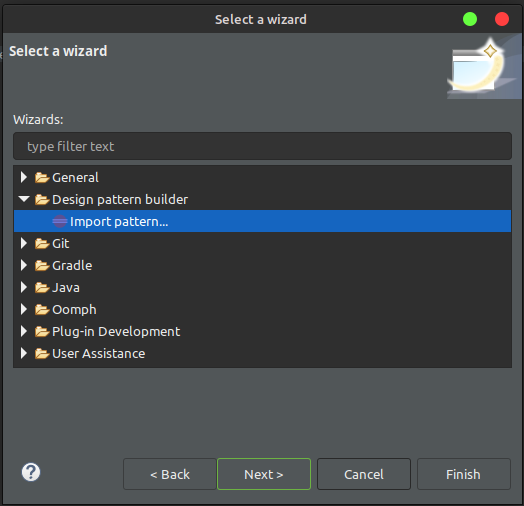
\includegraphics[width=1.0\textwidth]{Figures/open_wizard.png}
    \caption{Άνοιγμα οδηγού.}
    \label{fig:open_wizard}
\end{figure}
\begin{figure}[H]
    \centering
    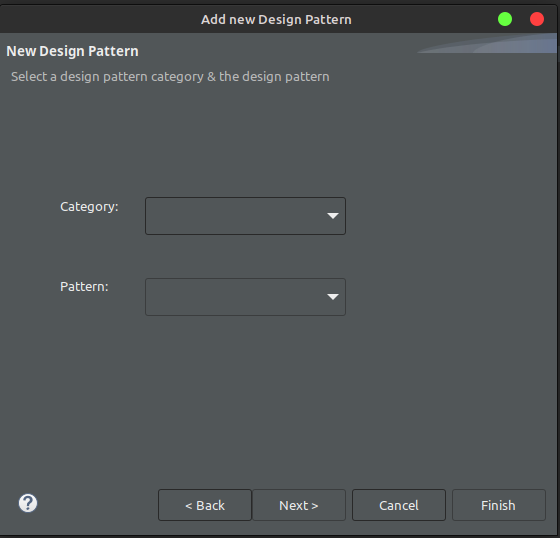
\includegraphics[width=1.0\textwidth]{Figures/select_pattern.png}
    \caption{Σελίδα επιλογής κατηγορίας \& μοτίβου.}
    \label{fig:select_pattern}
\end{figure}
Στη συνέχεια ο προγραμματιστής μπορεί να επιλέξει κατηγορία μοτίβου, αφού επιλέξει κατηγορία τότε θα γίνει διαθέσιμη και η επιλογή μοτίβου, 
αφού επιλέξει και μοτίβο τότε θα μπορεί να πλοηγηθεί στην επόμενη σελίδα του οδηγού, όπως φαίνεται στην εικόνα \ref{fig:select_pattern1}.
\begin{figure}[H]
    \centering
    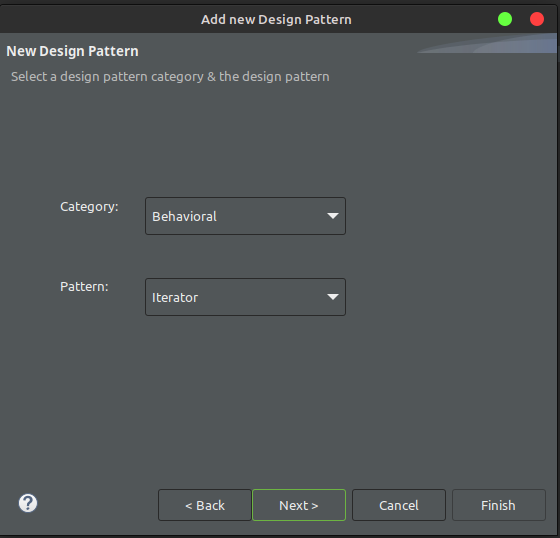
\includegraphics[width=1.0\textwidth]{Figures/select_pattern1.png}
    \caption{Επιλογή μοτίβου.}
    \label{fig:select_pattern1}
\end{figure}
Μόλις επιλέξει μοτίβο, ο οδηγός εμφανίζει τις κλάσεις και τις διεπαφές του μοτίβου. Στην εικόνα \ref{fig:classes_interfaces}, 
βλέπουμε ένα παράδειγμα για το μοτίβο Iterator \cite{GoF}. Ο προγραμματιστής στη συνέχεια, 
μπορεί είτε, να επεξεργαστεί κάποια κλάση ή διεπαφή, επιλέγοντας την από την λίστα και κάνοντας κλικ στο αντίστοιχο κουμπί, 
είτε, μα προσθέσει νέα κλάση εάν αυτό είναι επιτρεπτό, είτε, να ολοκληρώσει την διαδικασία χωρίς καμία τροποποίηση 
του μοτίβου κάνοντας κλικ στο κουμπί Finish.
\begin{figure}[H]
    \centering
    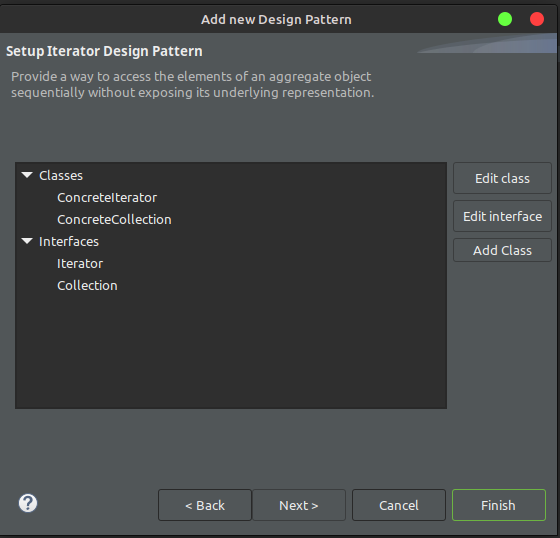
\includegraphics[width=1.0\textwidth]{Figures/classes_interfaces.png}
    \caption{Οι κλάσεις \& διεπαφές του μοτίβου Iterator.}
    \label{fig:classes_interfaces}
\end{figure}
Αφού ο προγραμματιστής, επιλέξει κάποια κλάση για να επεξεργαστεί, το σύστημα θα του εμφανίσει τη σελιδά \ref{fig:class_name}, 
όπου μπορεί να αλλάξει το όνομα της κλάσης και εάν πρόκειται για κλάση που έχει εισάγει ο χρήστης, 
να επιλέξει κάποια διεπαφή από τις διαθέσιμες για να υλοποιεί αυτή η κλάση. Επίσης μπορεί να σταματήσει εδώ την επεξεργασία της κλάσης, 
κάνοντας κλικ στο κουμπί Finish.
\begin{figure}[H]
    \centering
    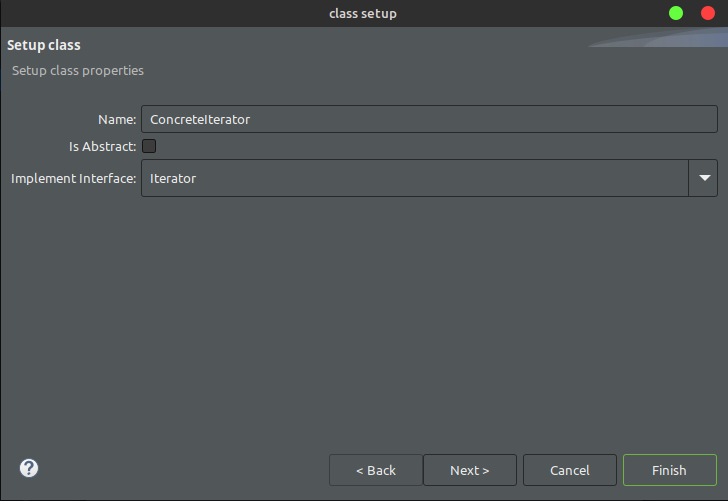
\includegraphics[width=1.0\textwidth]{Figures/class_name.png}
    \caption{Επεξεργασία ονόματος κλάσης.}
    \label{fig:class_name}
\end{figure}
Αφού έχει τροποποιήσει το όνομα της κλάσης, τότε στην επόμενη σελίδα \ref{fig:edit_fields}, 
έχει την δυνατότητα να τροποποιήσει τα πεδία της κλάσης, αλλάζοντας τις τιμές στα πεδία εισόδου, 
επίσης μπορεί να προσθέσει ή να διαγράψει κάποιο πεδίο όπως φαίνεται στην εικόνα \ref{fig:add_field}.
\begin{figure}[H]
    \centering
    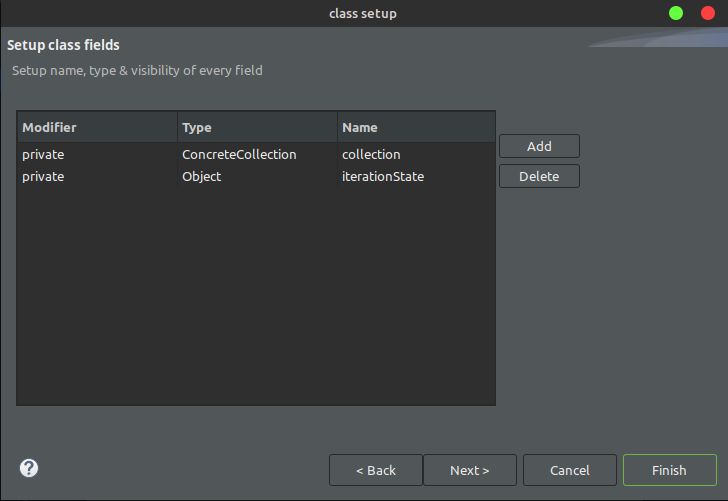
\includegraphics[width=1.0\textwidth]{Figures/edit_fields.png}
    \caption{Επεξεργασία πεδίων.}
    \label{fig:edit_fields}
\end{figure}
\begin{figure}[H]
    \centering
    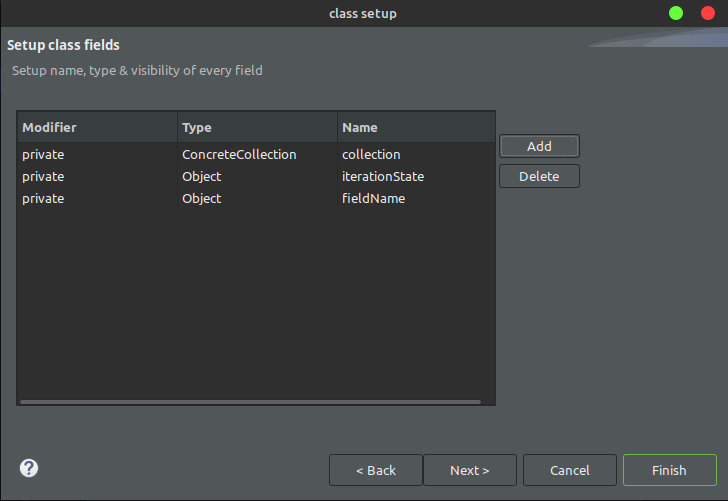
\includegraphics[width=1.0\textwidth]{Figures/add_field.png}
    \caption{Προσθήκη πεδίου.}
    \label{fig:add_field}
\end{figure}
Αφότου ο προγραμματιστής ολοκληρώσει την επεξεργασία των πεδίων, 
έχει την δυνατότητα να σταματήσει την επεξεργασία της κλάσης κάνοντας κλικ στο κουμπί finish, 
ή να συνεχίσει με την επεξεργασία των μεθόδων της κλάσης. Το σύστημα θα εμφανίσει την σελίδα \ref{fig:edit_class_methods}, 
όπου φαίνονται οι μέθοδοι της κλάσης που επεξεργάζεται ο προγραμματιστής. Δίνεται η δυνατότητα να τροποποιήσει κάποια μέθοδο, 
συμπληρώνοντας τα πεδία κειμένου. Επίσης μπορεί να προσθαφαιρέσει κάποια μέθοδο, όπως φαίνεται στην εικόνα \ref{fig:add_method}.
Τέλος μπορεί ο προγραμματιστής να επεξεργαστεί τις παραμέτρους κάποιας μεθόδου, κάνοντας κλικ στο κουμπί Edit Parameters.
\begin{figure}[H]
    \centering
    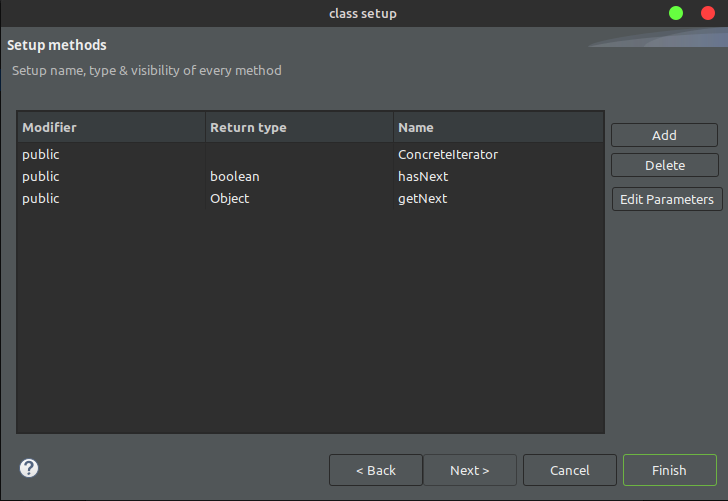
\includegraphics[width=1.0\textwidth]{Figures/edit_class_methods.png}
    \caption{Επεξεργασία μεθόδων κλάσης.}
    \label{fig:edit_class_methods}
\end{figure}
\begin{figure}[H]
    \centering
    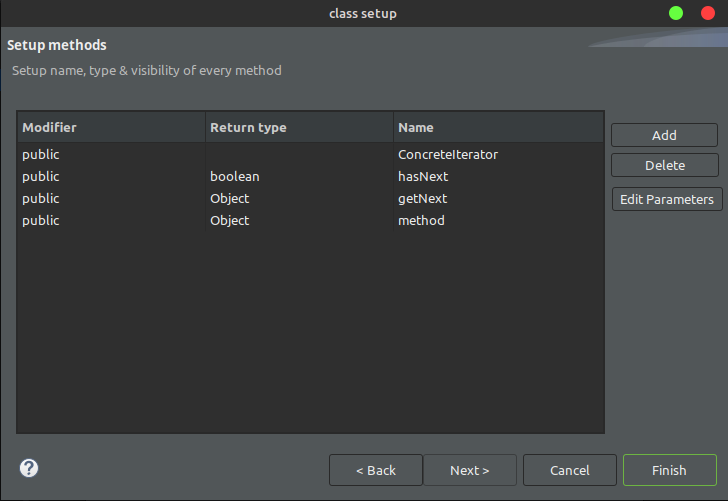
\includegraphics[width=1.0\textwidth]{Figures/add_method.png}
    \caption{Προσθήκη μεθόδου.}
    \label{fig:add_method}
\end{figure}
Μόλις ο προγραμματιστής πατήσει το κουμπί Edit Parameters, εμφανίζεται η σελίδα της εικόνας \ref{fig:edit_parameters}. 
Ο χρήστης μπορεί να προσθαφαιρέσει παραμέτρους, όπως στην εικόνα \ref{fig:add_parameters}, καθώς και να τις επεξεργαστεί.
\begin{figure}[H]
    \centering
    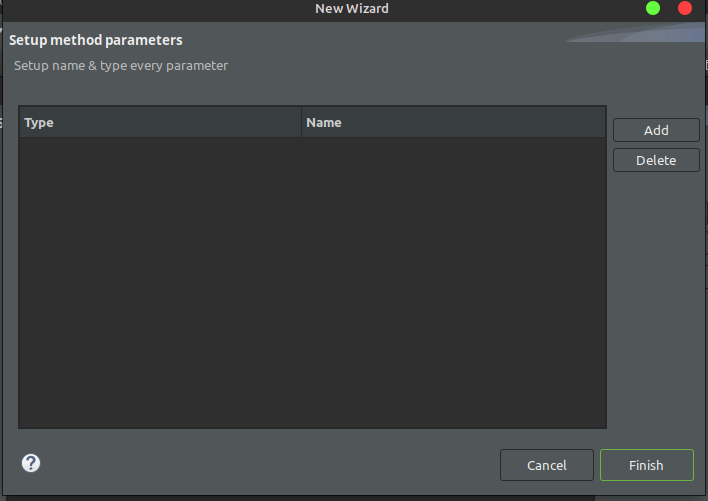
\includegraphics[width=1.0\textwidth]{Figures/edit_parameters.png}
    \caption{Επεξεργασία παραμέτρων μεθόδου.}
    \label{fig:edit_parameters}
\end{figure}
\begin{figure}[H]
    \centering
    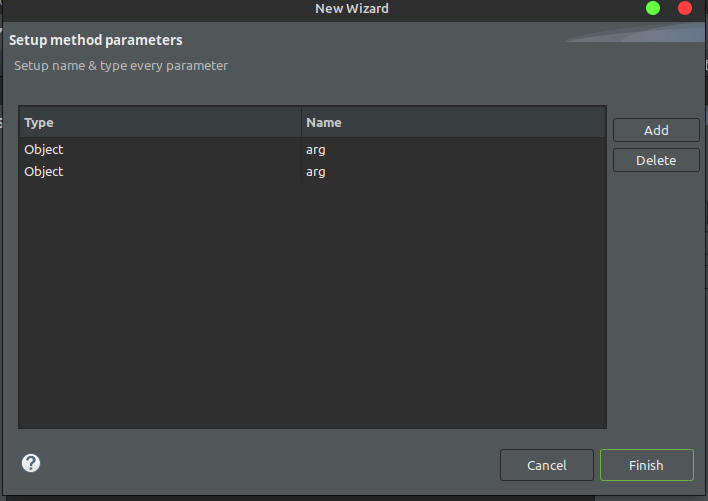
\includegraphics[width=1.0\textwidth]{Figures/add_parameters.png}
    \caption{Προσθήκη παραμέτρου.}
    \label{fig:add_parameters}
\end{figure}
Με αντίστοιχο τρόπο, ο προγραμματιστής έχει την δυνατότητα, να τροποποιήσει κάποια διεπαφή του μοτίβου, 
επιλέγοντας την διεπαφή που επιθυμεί και πατώντας το κουμπί Edit interface. Εμφανίζεται ένας αντίστοιχος οδηγός, ο οποίος φαίνεται 
στην εικόνα \ref{fig:edit_interface}, εδώ ο προγραμματιστής μπορεί να τροποποιήσει το όνομα της διεπαφής 
και να επιλέξει να τερματίσει την υπόλοιπη διαδικασία για την επεξεργασία της διεπαφής πατώντας το Finish, ή να συνεχίσει στην επόμενη 
σελίδα. Η οποία φαίνεται στην εικόνα \ref{fig:edit_interface_methods}, στην οποία μπορεί να 
επεξεργαστεί τις μεθόδους της διεπαφής όπως ακριβώς έκανε και με κάποια κλάση.
\begin{figure}[H]
    \centering
    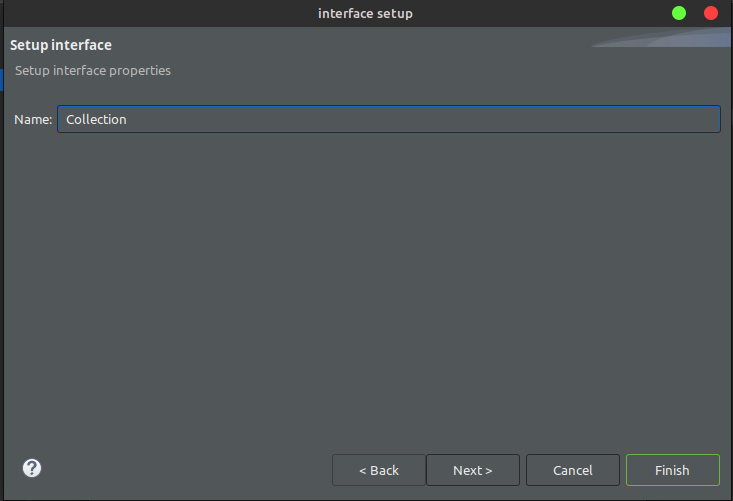
\includegraphics[width=1.0\textwidth]{Figures/edit_interface.png}
    \caption{Επεξεργασία ονόματος διεπαφής.}
    \label{fig:edit_interface}
\end{figure}
\begin{figure}[H]
    \centering
    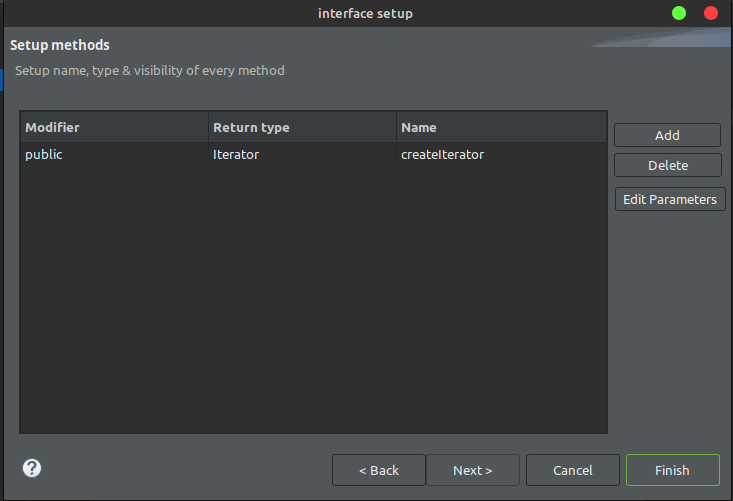
\includegraphics[width=1.0\textwidth]{Figures/edit_interface_methods.png}
    \caption{Επεξεργασία μεθόδων διεπαφής.}
    \label{fig:edit_interface_methods}
\end{figure}
Τέλος, μόλις ο προγραμματιστής κάνει τις αλλαγές που επιθυμεί, χρειάζεται να πατήσει το κουμπί Finish 
στην οθόνη \ref{fig:classes_interfaces} και το εργαλείο θα παράξει τα πηγαία αρχεία (\ref{fig:collection}, \ref{fig:concreteCollection}, \ref{fig:iterator}, \ref{fig:concreteIterator}) 
που αντιστοιχούν στο μοτίβο. 
Ο προγραμματιστής έχει την δυνατότητα να ακυρώσει και να τερματίσει τον οδηγό, οποιαδήποτε στιγμή επιθυμεί, πατώντας τα κουμπιά Cancel.
\begin{figure}[H]
    \centering
    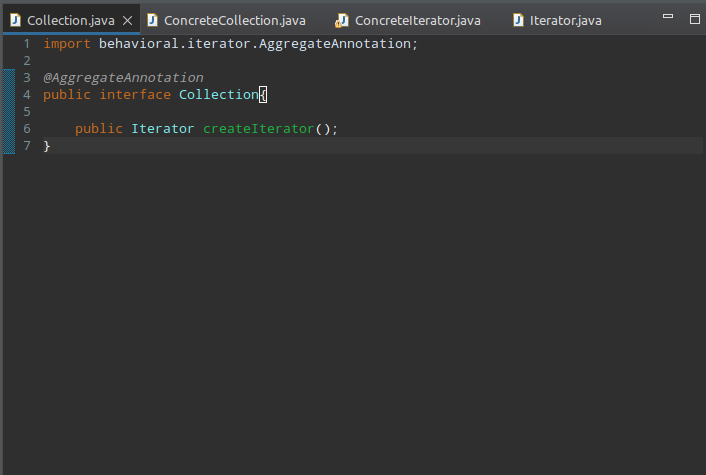
\includegraphics[width=1.0\textwidth]{Figures/collection.png}
    \caption{Διεπαφή Collection.}
    \label{fig:collection}
\end{figure}
\begin{figure}[H]
    \centering
    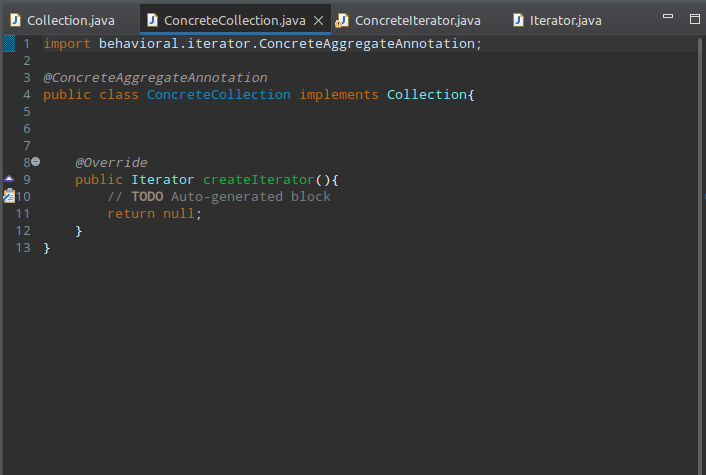
\includegraphics[width=1.0\textwidth]{Figures/concreteCollection.png}
    \caption{Κλάση ConcreteCollection.}
    \label{fig:concreteCollection}
\end{figure}
\begin{figure}[H]
    \centering
    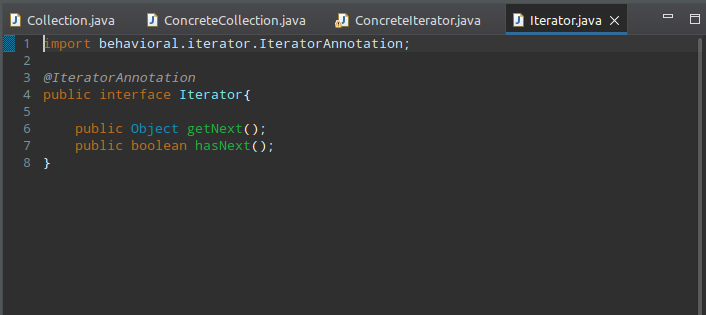
\includegraphics[width=1.0\textwidth]{Figures/iterator.png}
    \caption{Διεπαφή Iterator.}
    \label{fig:iterator}
\end{figure}
\begin{figure}[H]
    \centering
    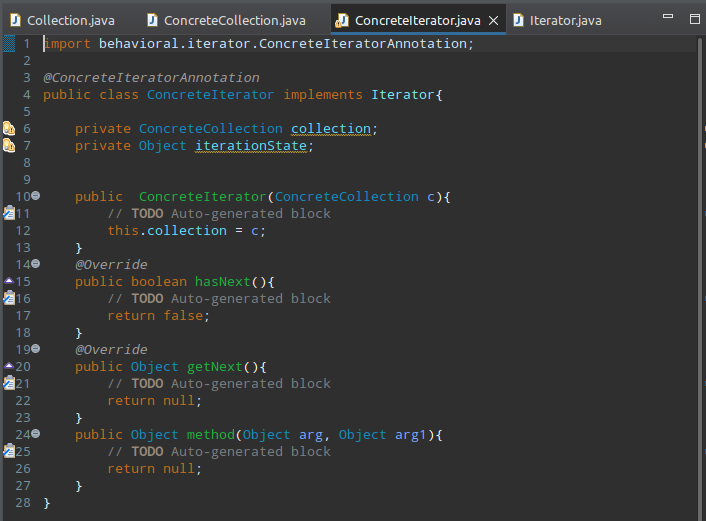
\includegraphics[width=1.0\textwidth]{Figures/concreteIterator.png}
    \caption{Κλάση ConcreteIterator.}
    \label{fig:concreteIterator}
\end{figure}
\chapter{Επίλογος}
\label{ch:epilogue}
\section{Σύνοψη και συμπεράσματα}
\label{sec:conclusion}
Στη διπλωματική αυτή δημιουργήθηκε ένα καινούριο εργαλείο 
με βασική λειτουργικότητα την ενσωμάτωση σχεδιαστικών μοτίβων σε πηγαίο κώδικα Java. 
Το εργαλείο βασίστηκε στα ήδη υπάρχοντα εργαλεία, Pattern Wizard, Patternbox, Design Pattern Automation Toolkit, καθώς και 
Alphaworks Design Pattern Toolkit \cite{PatternBox}, εξαλείφοντας  και συνεισφέροντας  σε βασικές 
τους ελλείψεις όπως η πληθώρα μοτίβων, την παραμετροποίηση των μοτίβων από τον χρήστη και τέλος, τον χαρακτηρισμό 
κάθε παραγόμενης κλάσης και διεπαφής, με την χρήση των annotations.\par
Επιπλέον, κάνοντας μία περιήγηση στο εργαλείο παρατηρούμε τα εξής: όλα τοποθετημένα στο ίδιο παράθυρο με τον κώδικα του χρήστη, 
καθώς πρόκειται για ένα εργαλείο το οποίο είναι επέκταση του περιβάλλοντος Eclipse.
Χάρη στον σχεδιασμό του, μπορεί κάποιος πολύ εύκολα να επεκτείνει τα διαθέσιμα μοτίβα 
και με άλλα μοτίβα εκτός από αυτά των GoF \cite{GoF}.\par Τέλος, η δυνατότητα των χρηστών να ελέγχουν ανά πάσα ώρα και στιγμή την πληροφορία 
που βρίσκεται μέσα στο εργαλείο. Καθώς, οι προσθήκες νέων μοτίβων από τον υπολογιστή του χρήστη όπως και η διαγραφή τους επιτρέπει, 
την εξατομικευμένη λειτουργία του. Έτσι, καλύπτονται πλήρως οι ανάγκες ενός προγραμματιστή ο οποίος έχει καλή γνώση των σχεδιαστικών μοτίβων.
\section{Μελλοντικές επεκτάσεις}
\label{sec:features}
Στην ενότητα, αυτή θα προταθούν μερικές επεκτάσεις του εργαλείου. Στο μέλλον, θα μπορούσε να προστεθεί η δυνατότητα 
να μπορεί κάποιος προγραμματιστής να αντιστοιχίσει κλάσεις και διεπαφές του μοτίβου με υπάρχουσες, 
οι οποίες βρίσκονται στο τρέχον έργο του προγραμματιστή. Έτσι, μπορεί να προσαρμόσει 
τις ήδη υπάρχουσες κλάσεις και διεπαφές στις ανάγκες του μοτίβου. Με αυτό τον τρόπο, δίνεται η δυνατότητα στον χρήστη
να εφαρμόσει διάφορα μοτίβα σε έργα τα οποία συντηρεί, αναδομώντας τα έργα αυτά και βελτιώνοντας τα.


% Εισαγωγή της βιβλιογραφίας
\addstarredchapterc{\bibname} % minitoc
\bibliographystyle{ieeetr}
\bibliography{Content/Bibliography}

% Προαιρετικά, μπορείτε να εισάγετε παραρτήματα
\appendix
\chapter{Τίτλος πρώτου παραρτήματος}
\label{app:FirstAppendix}

Εδώ είναι ο χώρος του πρώτου Παραρτήματος.

\begin{table}[h]
	\centering
	\caption{Πίνακας Παραρτήματος.}
	\label{tab:AppendixTable}
	\begin{tabular}{l l l l l}
		\hline
		~ & ~ & Sample Mean & ~ & 95\% Confidence Interval \\
		\hline
		1 process & ~ & $3.640966$  & ~ & $0.100136$ \\
		4 processes & ~ & $1.053655$  & ~ & $0.037212$ \\
		8 processes & ~ & $0.610223$  & ~ & $0.023470$ \\
		16 processes & ~ & $0.357321$  & ~ & $0.014783$ \\
		32 processes & ~ & $0.227180$  & ~ & $0.016923$ \\
		\hline
	\end{tabular}
\end{table}
%\chapter{Τίτλος δεύτερου παραρτήματος}
\label{app:SecondAppendix}

\section{Τίτλος πρώτης ενότητας}
\label{sec:FirstSection}
Εδώ είναι ο χώρος της πρώτης ενότητας του δεύτερου Παραρτήματος.

\section{Τίτλος δεύτερης ενότητας}
\label{sec:SecondSection}
Εδώ είναι ο χώρος της δεύτερης ενότητας του δεύτερου Παραρτήματος.
%\chapter{Τίτλος τρίτου παραρτήματος}
\label{app:ThirdAppendix}

Εδώ είναι ο χώρος του τρίτου Παραρτήματος.

\begin{figure}[h]
	\centering
	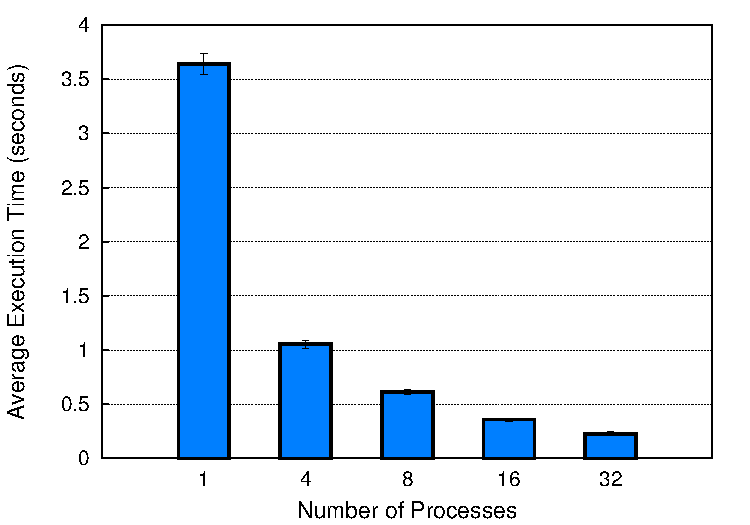
\includegraphics[width=0.65\textwidth]{Figures/MatrixMultiplication.pdf}
	\caption{Εικόνα Παραρτήματος.}
	\label{fig:AppendixFigure}
\end{figure}


% Εκτύπωση του ευρετηρίου (προαιρετικό)
\printindex


\end{document}
